\documentclass[11pt,a4paper,oneside]{article}
\usepackage{xcolor}
\usepackage{listings}
\usepackage{mathptmx}
\usepackage[cm]{fullpage}
\usepackage{hyperref}
\usepackage{graphicx}
\usepackage{caption}
\linespread{1.3}

\hypersetup{
  pdfborder={0 0 0},
  colorlinks=true,
  linkcolor=blue,
  urlcolor=cyan
}

\urlstyle{same}

\begin{document}

\definecolor{lightyellow}{rgb}{1,1,0.8}
\lstset{backgroundcolor=\color{lightyellow},
  basicstyle=\fontsize{9}{11}\ttfamily,
  keepspaces=true,
  showspaces=false,
  showstringspaces=false,
  columns=fullflexible }

\setcounter{secnumdepth}{4}
\setcounter{tocdepth}{4}

\title{RZ/A2M for Zephyr Release Notes v0.2alpha}
\author{EPAM Systems}
\date{December, 2023}

\maketitle

\tableofcontents

\clearpage

\section{Preface}\label{preface}

This release introduces the basic support for the RZ/A2M board. It
includes a set of HW drivers which allows Zephyr to run on the target
board.

\section{Scope of delivery}\label{scope-of-delivery}

The release includes the following items:

\begin{itemize}
\item This Release Notes.
\item Zephyr repository with the source code set of drivers for RZ/A2M support integrated.
\end{itemize}

\section{Gettig source code}\label{gettig-source-code}

Follow Zephyr Getting Started Guide:
\url{https://docs.zephyrproject.org/latest/develop/getting_started/index.html},
but change the one step from ``\emph{Get the Zephyr source code}'':

Instead of using this command \emph{west init
\textasciitilde/zephyrproject} use the next one from your working
directory:

\begin{lstlisting}
west init -m git@gitbud.epam.com:rec-rzzp/zephyr.git --mr release-0.2alpha zephyr_rza2m
cd zephyr_rza2m/zephyr
\end{lstlisting}

Cloning GIT repo for the first time requires SSH keys to be
registration. Please follow this guide for the detailed instructions:

\url{https://gitbud.epam.com/help/user/ssh.md}

\section{Board initial configuration}\label{board-initial-configuration}

Hardware used for testing: RZ/A2M EVK board (RTK7921053S000000BE)
\url{https://www.renesas.com/us/en/products/microcontrollers-microprocessors/rz-mpus/rza2m-evkit-rza2m-evaluation-kit}.

The initial Board Configuration is shown on the following schema:

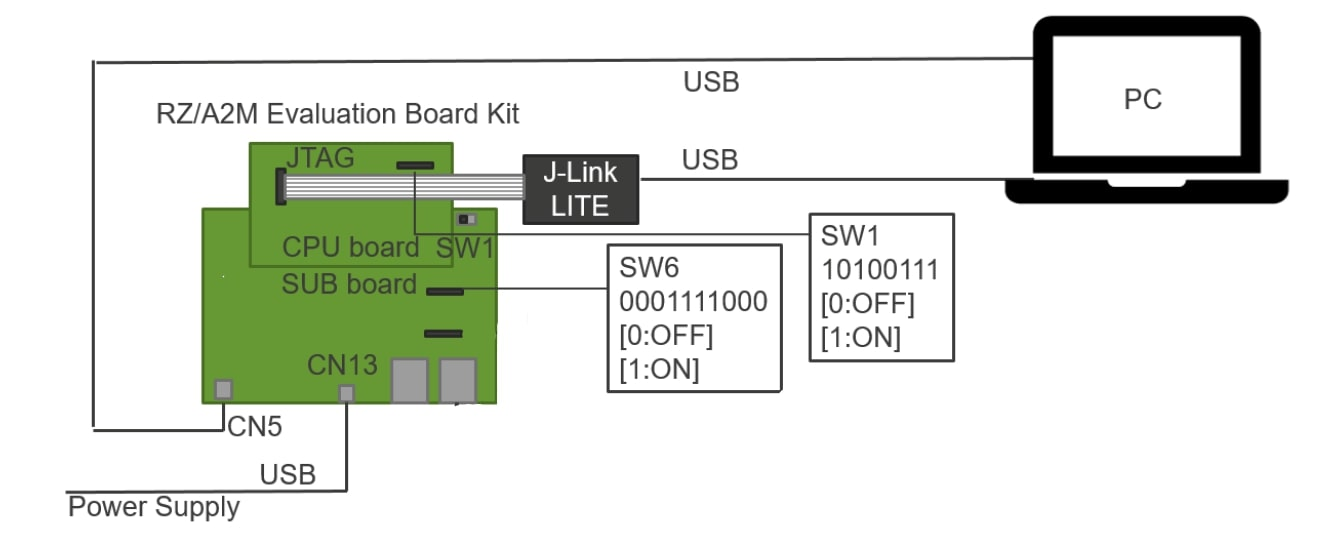
\includegraphics[width=6.66667in,height=2.6875in]{./media/image4.jpg}

\begin{enumerate}
\def\labelenumi{\arabic{enumi}.}
\item
  Confirm Power switch (SW1) on SUB board is ON (left).
\item
  Connect CPU board and SUB board.
\item
  Set SW1 on CPU board to 10100111.
\item
  Set SW6 on SUB board to 0001111000.
\item
  Connect J-Link LITE to JTAG connector on CPU board.
\item
  Connect the USB cable from J-Link LITE to a spare USB port on your PC.
\item
  Connect the USB cable form CN5 on SUB board to a spare USB port on
  your PC.
\end{enumerate}

Also, please confirm that the Jumpers on the CPU and SUBBOARD are set to
the following configuration:

1.JP3 on the CPU board is disconnected.

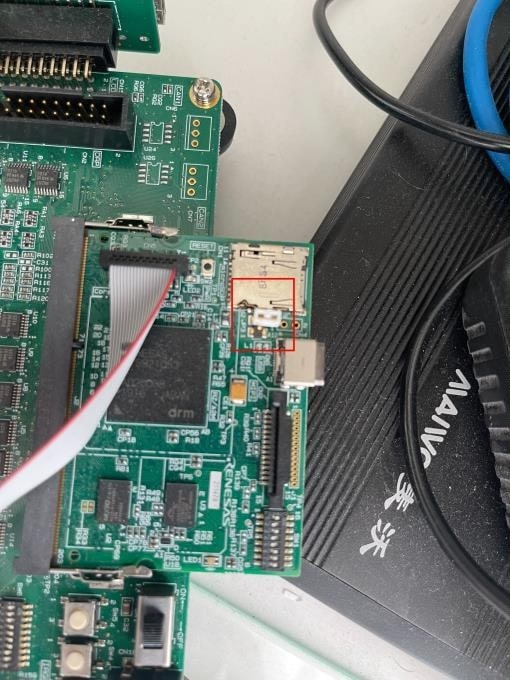
\includegraphics[width=2.55208in,height=3.40278in]{./media/image.jpg}

2.JP1\_2 on the SUBBOARD is connected to JP2

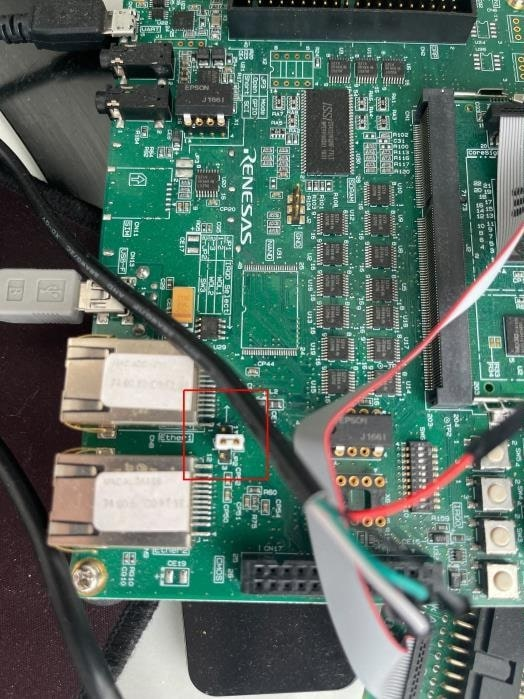
\includegraphics[width=2.625in,height=3.5in]{./media/image2.jpg}

Set up the PC environment:

\begin{enumerate}
\def\labelenumi{\arabic{enumi}.}
\item
  Download the source code using instructions from
  \hyperref[gettig-source-code]{Getting source code}.
\item
  Connect Segger Jlink to CN5 (Coresight) on the Main board to the USB
  port in your PC.
\item
  Connect miniUSB (CN5 on the Subboard with marking UART) to the USB
  port on your PC.
\item
  Proceed with steps to find tty device: run command:
  \colorbox{lightgray}{dmesg} after connecting CN5 Subboard port to your PC.
\item
  Open 2 terminal windows on your PC.
\end{enumerate}

On the first terminal run:
\begin{lstlisting}
sudo minicom -D /dev/ttyXXX
\end{lstlisting}

NOTE: in most cases device will have the name /dev/ttyACM0

NOTE: minicom is the Serial console program. It can be installed using
your native packaging system. For example, to install minicom on Ubuntu
you can use the following command:

\begin{lstlisting}
sudo apt install minicom
\end{lstlisting}

If you use alternatives for minicom, please set the following connection
settings:

Communication speed: 115,200bps

Communication settings:

Data length: 8 bits
Parity: None

Stop bits: 1 bit

Flow control: None

On the second terminal the debug session can be started using commands:
\colorbox{lightgray}{west debug} and then \colorbox{lightgray}{continue}.

Test result will appear in the minicom window.

For example, to build a Zephyr image with the tests image, please use
the following command:

\begin{lstlisting}
west build -p always -b rz_a2m tests/drivers/pinctrl/rz_a2m
\end{lstlisting}

Start the debugging session using the procedure below:

1) Attach RZ/A2M board to the PC using both JLink and UART connectors.

2) Make sure that the board is powered off.

3) Power on the board using SW1.

4) Execute the following steps to clean up the flash drive:

\begin{lstlisting}
/opt/SEGGER/JLink_V792a/JLinkExe -nogui 1 -if swd -speed 15000 -device R7S921053VCBG\
-nogui 1
J-Link> exec EnableEraseAllFlashBanks
J-Link> erase 0x20000000,0x20002000
\end{lstlisting}

See \hyperref[building-and-flashing]{Building and Flashing} section
for the details.

5) Switch the board off then on using SW1 switch.

6) Identify ttyXXX device.

Run the command: \colorbox{lightgray}{dmesg}

After plugging in the UART USB connector, y you should find information
similar to the format below:

\begin{lstlisting}
[2163454.393244] usb 3-1: USB disconnect, device number 106
[2163456.501104] usb 3-1: new full-speed USB device number 108 using xhci_hcd
[2163456.652778] usb 3-1: New USB device found, idVendor=045b, idProduct=8500,\
bcdDevice=10.00
[2163456.652802] usb 3-1: New USB device strings: Mfr=1, Product=2, SerialNumber=5
[2163456.652807] usb 3-1: Product: CDC USB Demonstration
[2163456.652811] usb 3-1: Manufacturer: Renesas Electronics Corporation
[2163456.652814] usb 3-1: SerialNumber: 0000000000001
[2163456.655410] cdc_acm 3-1:1.0: ttyACM0: USB ACM device
\end{lstlisting}

According to the last line, you should use /dev/ttyACM0 to connect to
the board Serial Console.

Connect to the Serial console:

\begin{lstlisting}
sudo minicom -D /dev/ttyACM0
\end{lstlisting}

Start the debug session (see Section 5. Building and Flashing of the
Release Notes for the details) by running command: \colorbox{lightgray}{west debug}

Which will upload image to the target board using JLink console and open
the Debug session.

Once in the Debug session, run the command: \colorbox{lightgray}{continue} to proceed.

The results should then appear on the UART console.

These steps are applicable for all tests and sample programs.

\section{Building and Flashing}\label{building-and-flashing}

RZ/A2M board has Segger Jlink connected to the pc which can be used for
debugging purposes and to upload image to the board.

Preparations for the RZ/A2M board debug process:

\begin{enumerate}
\def\labelenumi{\arabic{enumi})}
\item
  Attach RZ/A2M board to the PC using both JLink and UART connectors.
\item
  Power on the board.
\item
  Identify ttyXXX device. Run the command:
\end{enumerate}

\begin{lstlisting}
dmesg
\end{lstlisting}

After plugging in the UART USB connector (CN5 connector on the SUBBOARD)
to your PC, you should find information similar to the format below:

\begin{lstlisting}
[2163454.393244] usb 3-1: USB disconnect, device number 106
[2163456.501104] usb 3-1: new full-speed USB device number 108 using xhci_hcd
[2163456.652778] usb 3-1: New USB device found, idVendor=045b, idProduct=8500,\
bcdDevice=10.00
[2163456.652802] usb 3-1: New USB device strings: Mfr=1, Product=2, SerialNumber=5
[2163456.652807] usb 3-1: Product: CDC USB Demonstration
[2163456.652811] usb 3-1: Manufacturer: Renesas Electronics Corporation
[2163456.652814] usb 3-1: SerialNumber: 0000000000001
[2163456.655410] cdc_acm 3-1:1.0: ttyACM0: USB ACM device
\end{lstlisting}

According to the last line, you should use /dev/ttyACM0 to connect to
the board Serial Console.

\begin{enumerate}
\def\labelenumi{\arabic{enumi})}
\setcounter{enumi}{3}
\item
  Connect to the Serial console:
\end{enumerate}

\begin{lstlisting}
sudo minicom -D /dev/ttyACM0
\end{lstlisting}

Let's take sample to show how this can be done:

\begin{lstlisting}
west build -b rz_a2m -p always samples/basic/blinky
\end{lstlisting}

\# \colorbox{lightgray}{-p always} instructs west to recompile project each time. It is
preferable to use this flag

The result build image is placed in build/zephyr/zephyr.elf

To start debugging section using SEGGER JLink the following command
should be executed:

\begin{lstlisting}
west debug
\end{lstlisting}

\# To use different gdb client the following flag should be added
-\/-gdb=gdb-multiarch

This command will upload Zephyr image to RAM and start a debug session
with PC on the first instruction. Please refer to
\hyperref[appendix-1.-gdb-debug-session-output]{Appendix 1} for the gdb
session output example.

To continue execution enter \colorbox{lightgray}{continue} command to the GDB console.

Details about GDB debugging process can be found in the following
document:

\url{https://ftp.gnu.org/old-gnu/Manuals/gdb/html_node/gdb_toc.html}

NOTE: Using SEGGER JLink requires software to be installed. Please
Download SW package from the following location:
\url{https://www.segger.com/downloads/jlink/} and follow installation
instructions.

The result will be gdb session via JLink server. Zephyr image will be
loaded to RAM using Jlink.

Image can also be uploaded to the internal flash memory using the
following command:

\begin{lstlisting}
west flash
\end{lstlisting}

Please note that you should enable \colorbox{lightgray}{CONFIG\_XIP=y} so the board can
start from flash memory.

After that the board will start from flash after each reboot.

\textbf{NOTE:} If it is needed to cleanup the Serial Flash on the board the following
steps can be done:

\begin{lstlisting}
/opt/SEGGER/JLink_V792a/JLinkExe -nogui 1 -if swd -speed 15000 -device
R7S921053VCBG -nogui 1
J-Link> exec EnableEraseAllFlashBanks
J-Link> erase 0x20000000,0x20002000
\end{lstlisting}

\section{Features support implemented}\label{features-support-implemented}

\subsection{Pinctrl and GPIO support}\label{pinctrl-and-gpio-support}

Renesas RZ/A2 combined Pin Function and GPIO Controller node Pin
multiplexing and GPIO configuration is performed on a per-pin basis.
Each port features up to 8 pins, each of them configurable for GPIO
function (port mode) or in alternate function mode.

Up to 8 different alternate function modes exist for each single pin.

It is embedded to the basic RZ/A2M support and can be tested using the
following samples:

\begin{lstlisting}
west build -p always -b rz_a2m samples/basic/blinky
\end{lstlisting}

After building the image can be started by using command \colorbox{lightgray}{west debug}
and then \colorbox{lightgray}{continue} from the GDB. Please refer to
\hyperref[building-and-flashing]{Building and Flashing} for the
details.

This sample uses GPIO pins to blink LED forever on the main board.
Please follow the link
\url{https://docs.zephyrproject.org/latest/samples/basic/blinky/README.html}
for additional information.

NOTE: Running the \textquotesingle blinky\textquotesingle{} sample will
cause the green LED (LED1) on the main board to blink.

And

\begin{lstlisting}
west build -p always -b rz_a2m samples/basic/button
\end{lstlisting}

This test does gpio configuration for SW4 button to send interrupt and
blinks with LED each time the button is pressed.

Please follow the link
\url{https://docs.zephyrproject.org/latest/samples/basic/button/README.html}
for additional information.

After building the image can be started by using command \colorbox{lightgray}{west debug}
and then \colorbox{lightgray}{continue} from the GDB. Please refer to
\hyperref[building-and-flashing]{Building and Flashing} for the
details.

NOTE: Running the \textquotesingle button\textquotesingle{} sample will
cause the green LED (LED1) on the main board to turn on. It will turn
off when the button (SW4) is pressed.

Pinctrl function set can be tested using the following test:

\begin{lstlisting}
west build -p always -b rz_a2m tests/drivers/pinctrl/rz_a2m
\end{lstlisting}

This is a new test for the pinctrl functionality written for the RZ/A2M
board which validates Pinctrl API. It performs the following tests:

\begin{itemize}
\item
  test\_dt\_extract -- validates extraction of the Pinctrl configuration
  from the Device Tree bindings and confirms that pinctrl configuration
  can be retrieved.
\item
  test\_lookup\_state -- validates pinctrl\_lookup\_state API call to
  retrieve the default state configuration.
\item
  test\_apply\_state -- validates pinctl\_apply\_state API call to apply
  state configuration.
\end{itemize}

The following documentation:
\url{https://docs.zephyrproject.org/latest/hardware/pinctrl/index.html}
provides the details about Pinctrl API defined in Zephyr.

After building the image can be started by using command \colorbox{lightgray}{west debug}
and then \colorbox{lightgray}{continue} from the GDB. Please refer to
\hyperref[building-and-flashing]{Building and Flashing} for the
details.

The result is the following:

\begin{lstlisting}
CTRL-A Z for help 115200 8N1 NOR
Minicom 2.7.1 VT102 Offline ttyACM0

*** Booting Zephyr OS build zephyr-v3.4.0-2118-g461885a11a63 ***
Running TESTSUITE p_rza2_suite
===================================================================
START - test_apply_state
PASS - test_apply_state in 0.001 seconds
===================================================================
START - test_dt_extract
PASS - test_dt_extract in 0.001 seconds
===================================================================
START - test_lookup_state
PASS - test_lookup_state in 0.001 seconds
===================================================================
TESTSUITE p_rza2_suite succeeded

------- TESTSUITE SUMMARY START -------

SUITE PASS - 100.00% [p_rza2_suite]: pass = 3, fail = 0, skip =
0, total = 3 duration = 0.003 seconds

- PASS - [p_rza2_suite.test_apply_state] duration = 0.001 seconds
- PASS - [p_rza2_suite.test_dt_extract] duration = 0.001 seconds
- PASS - [p_rza2_suite.test_lookup_state] duration = 0.001
seconds

------- TESTSUITE SUMMARY END -------
===================================================================

PROJECT EXECUTION SUCCESSFUL
\end{lstlisting}

\subsection{Clock driver support}\label{clock-driver-support}

The clock control API provides access to clocks in the system, including
the ability to turn them on and off.

The driver is based on the Renesas R-Car CPG driver core and implements
only a few API calls:
\begin{itemize}
  \item
    clock\_control\_on
  \item
    clock\_control\_off
  \item
    clock\_control\_get\_rate
  \item
    clock\_control\_set\_rate
\end{itemize}

Notes:
\begin{itemize}
  \item
    on/off works only for Module clocks; Core clocks can be disabled due to HW restrictions.
  \item
    set\_rate can only work with Core clocks.
  \item
    I, B, and P1 Core clocks have been set to the maximum possible frequency by default in the
    CPG init function: 528, 132, and 66, respectively.
  \item
    CLKIO is enabled by default as a low-level output, and it isn't configurable.
  \item
    The B Core clock is chosen as the default output for CLKIO. This selection occurs only when
    XIP isn't chosen because the register that selects the clock for CLKIO can only be accessed from
    On-Chip RAM code. It should be fixed in scope of \url{https://jiraeu.epam.com/browse/RECRZZP-81}.
\end{itemize}

Detailed information about these calls can be found using the next link:
\url{https://docs.zephyrproject.org/latest/hardware/peripherals/clock_control.html}

\subsection{UART support}\label{uart-support}

Zephyr provides three different ways to access the UART peripheral.
Depending on the method, different API functions are used according to
below sections:

\begin{itemize}
\item
  Polling API
\item
  Interrupt-driven API
\item
  Asynchronous API using Direct Memory Access (DMA)
\end{itemize}

This driver can be checked the following way:

Connect to the board serial using:

\begin{lstlisting}
sudo minicom -D /dev/ttyACM0
\end{lstlisting}

The correct tty device can be got from dmesg. The following message
should appear when attaching serial console port to the PC:

\begin{lstlisting}
[1758184.097866] usb 3-1: New USB device found, idVendor=045b, idProduct=8500,\
bcdDevice=10.00
[1758184.097875] usb 3-1: New USB device strings: Mfr=1, Product=2, SerialNumber=5
[1758184.097878] usb 3-1: Product: CDC USB Demonstration
[1758184.097880] usb 3-1: Manufacturer: Renesas Electronics Corporation
[1758184.097882] usb 3-1: SerialNumber: 0000000000001
[1758184.099855] cdc_acm 3-1:1.0: ttyACM0: USB ACM device
\end{lstlisting}

And start zephyr image, for example:

\begin{lstlisting}
west build -p always -b rz_a2m /samples/basic/button
\end{lstlisting}

After building the image can be started by using command \colorbox{lightgray}{west debug}
and then \colorbox{lightgray}{continue} from the GDB. Please refer to
\hyperref[building-and-flashing]{Building and Flashing} for the
details.

Output can be seen on the minicom.

Testing UART using basic tests can be done as follows:

\begin{lstlisting}
west build -p always -b rz_a2m tests/drivers/uart/uart_basic_api/
\end{lstlisting}

After building the image can be started by using command \colorbox{lightgray}{west debug}
and then \colorbox{lightgray}{continue} from the GDB. Please refer to
\hyperref[building-and-flashing]{Building and Flashing} for the
details.

This test performs validation in the uart basic API described in
\url{https://docs.zephyrproject.org/latest/hardware/peripherals/uart.html}

This test is the basic uart API test for Zephyr and validates the basic
configuration and communication API for uart.

This has the following source files included which can be found in the
\begin{lstlisting}
tests/drivers/uart/uart_basic_api/src
\end{lstlisting}
directory:

\begin{tabular}{|l|l|}
  \hline
  main.c & Main test source file for uart test \\
  \hline
  test\_uart\_config.c & verify UART configure API settings \\
  \hline
  test\_uart\_fifo.c & verify UART works well in fifo mode \\
  \hline
  test\_uart\_pending.c & test UART uart\_irq\_is\_pending() \\
  \hline
  test\_uart\_poll.c & Verify UART poll api \\
  \hline
\end{tabular}

NOTE: The details about the test scenario can be found in the comment on
the top of each source file.

NOTE: test\_uart\_poll.c doesn't have a comment with the test scenario.
It is verifying that uart polling works properly. After starting it
request user to put some symbols to the UART console connected then
prints it to the console. Send \textbackslash n (Enter) to finish the
test.

The result is the following:

\begin{lstlisting}
*** Booting Zephyr OS build zephyr-v3.4.0-2132-g784951b7863d ***
Running TESTSUITE uart_basic_api
===================================================================
START - test_uart_config_get
This is a configure_gMM- test_uart_config_get in 0.003 seconds
===================================================================
START - test_uart_cMM- test_uart_configure in 0.001 seconds
===================================================================
START - test_uart_fifo_fill
TMhiinsi ciosm 2a. 8FIFO test.
PASS - test_uart_fifo_fill in 0.501 seconds
===================================================================
START - test_uart_fifo_read
Please send characters to serial console
PASS - test_uart_fifo_read in 2.475 seconds
===================================================================
START - test_uart_poll_in
Please send characters to serial console
PASS - test_uart_poll_in in 2.011 seconds
===================================================================
START - test_uart_poll_out
This is a POLL test.
PASS - test_uart_poll_out in 0.002 seconds
===================================================================
TESTSUITE uart_basic_api succeeded
Running TESTSUITE uart_basic_api_pending
===================================================================
START - test_uart_pending
Please send characters to serial console
PASS - test_uart_pending in 2.079 seconds
===================================================================
TESTSUITE uart_basic_api_pending succeeded

------- TESTSUITE SUMMARY START -------

SUITE PASS - 100.00% [uart_basic_api]: pass = 6, fail = 0, skip =
0, total = 6 duration = 4.993 seconds
- PASS - [uart_basic_api.test_uart_config_get] duration = 0.003 seconds
- PASS - [uart_basic_api.test_uart_configure] duration = 0.001 seconds
- PASS - [uart_basic_api.test_uart_fifo_fill] duration = 0.501 seconds
- PASS - [uart_basic_api.test_uart_fifo_read] duration = 2.475 seconds
- PASS - [uart_basic_api.test_uart_poll_in] duration = 2.011 seconds
- PASS - [uart_basic_api.test_uart_poll_out] duration = 0.002 seconds

SUITE PASS - 100.00% [uart_basic_api_pending]: pass = 1, fail =
0, skip = 0, total = 1 duration = 2.079 seconds
- PASS - [uart_basic_api_pending.test_uart_pending] duration =
2.079 seconds

------- TESTSUITE SUMMARY END -------

===================================================================
PROJECT EXECUTION SUCCESSFUL
\end{lstlisting}

To test UART async API via DMA please use the following command:

\begin{lstlisting}
west build -p always -b rz_a2m tests/drivers/uart/uart_async_api/
\end{lstlisting}

After building the image can be started by using command \colorbox{lightgray}{west debug}
and then \colorbox{lightgray}{continue} from the GDB. Please refer to
\hyperref[building-and-flashing]{Building and Flashing} for
the details.

Before running test application, please check pins 9 and 10 on CN17 Connector should be connected.

Please proceed with the following steps to prepare setup for the
testing:

\begin{enumerate}
\def\labelenumi{\arabic{enumi})}
\item
  Turn Off the board.
\item
  Ensure that SW6\_4 is ``OFF'' on the SUBBOARD.
\end{enumerate}

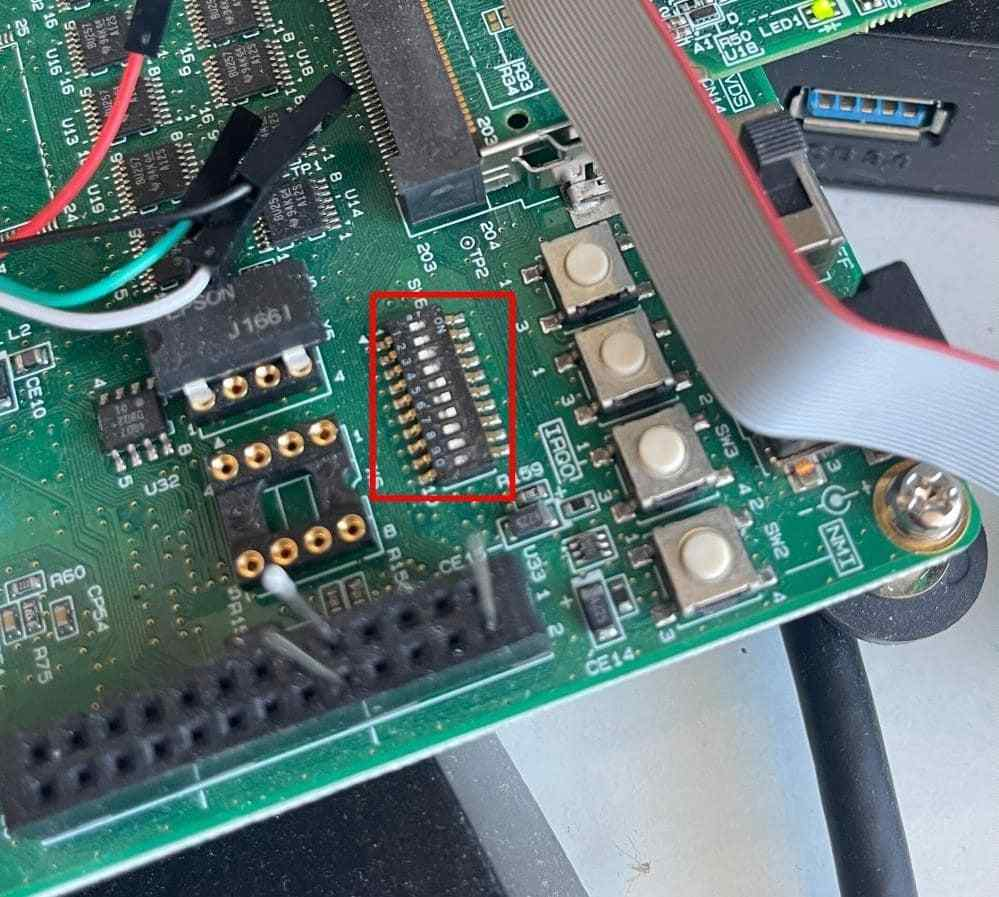
\includegraphics[width=5in,height=4.48958in]{./media/image3.jpg}

\begin{enumerate}
\def\labelenumi{\arabic{enumi})}
\setcounter{enumi}{2}
\item
  Connect pin 9 to pin 10 on CN17 connector.
\end{enumerate}

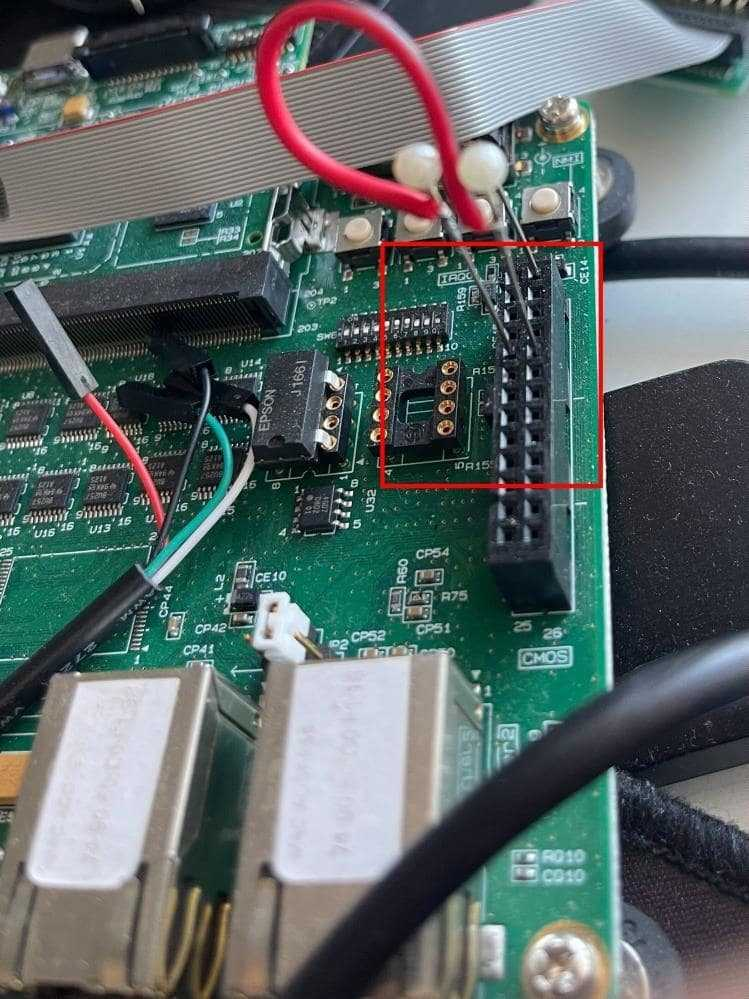
\includegraphics[width=3.75in,height=5in]{./media/image31.jpg}

\begin{enumerate}
\def\labelenumi{\arabic{enumi})}
\setcounter{enumi}{3}
\item
  Turn on the board and start the test.
\end{enumerate}

NOTE: Don't forget to switch SW6\_4 back to ON after the test is
finished.

This test is part of the Zephyr test collection. It verifies the work of
the Zephyr Async API. Please see the link:
\url{https://docs.zephyrproject.org/apidoc/latest/group__uart__async.html}
for the API definitions.

In current implementation the following tests are passed:

\begin{itemize}
\item
  test\_chained\_write -- executes UART transfer for a chained buffers
  using DMA channels and verify that buffers were passed successfully.
\end{itemize}

\begin{itemize}
\item
  test\_read\_abort -- validates transfer abort work. Performs UART
  async transfer and then validates transfer abort then timeout was
  reached.
\end{itemize}

\begin{itemize}
\item
  test\_single\_read -- validates async read and write operations.
\end{itemize}

\begin{itemize}
\item
  test\_forever\_timeout -- validates the scenario when the timeout
  FOREVER was set. Checks if transmission is still going after some
  time.
\end{itemize}

The result is the following:

\begin{lstlisting}
*** Booting Zephyr OS build zephyr-v3.3.0-7341-ge263117b9e77 ***

Running TESTSUITE uart_async_chain_read
===================================================================
START - test_chained_read
SKIP - test_chained_read in 0.001 seconds
===================================================================
TESTSUITE uart_async_chain_read succeeded
Running TESTSUITE uart_async_chain_write
===================================================================
START - test_chained_write
PASS - test_chained_write in 0.002 seconds
===================================================================
TESTSUITE uart_async_chain_write succeeded
Running TESTSUITE uart_async_double_buf
===================================================================
START - test_double_buffer
SKIP - test_double_buffer in 0.001 seconds
===================================================================
TESTSUITE uart_async_double_buf succeeded
Running TESTSUITE uart_async_long_buf
===================================================================
START - test_long_buffers
SKIP - test_long_buffers in 0.001 seconds
===================================================================
TESTSUITE uart_async_long_buf succeeded
Running TESTSUITE uart_async_multi_rx
===================================================================
START - test_multiple_rx_enable
SKIP - test_multiple_rx_enable in 0.001 seconds
===================================================================
TESTSUITE uart_async_multi_rx succeeded
Running TESTSUITE uart_async_read_abort
===================================================================
START - test_read_abort
PASS - test_read_abort in 1.118 seconds
===================================================================
TESTSUITE uart_async_read_abort succeeded
Running TESTSUITE uart_async_single_read
===================================================================
START - test_single_read
PASS - test_single_read in 0.351 seconds
===================================================================
TESTSUITE uart_async_single_read succeeded
Running TESTSUITE uart_async_timeout
===================================================================
START - test_forever_timeout
PASS - test_forever_timeout in 3.001 seconds
===================================================================
TESTSUITE uart_async_timeout succeeded
Running TESTSUITE uart_async_write_abort
===================================================================
START - test_write_abort
SKIP - test_write_abort in 0.001 seconds
===================================================================
TESTSUITE uart_async_write_abort succeeded

------- TESTSUITE SUMMARY START -------

SUITE SKIP - 0.00% [uart_async_chain_read]: pass = 0, fail = 0,
skip = 1, total = 1 duration = 0.001 seconds
- SKIP - [uart_async_chain_read.test_chained_read] duration =
0.001 seconds

SUITE PASS - 100.00% [uart_async_chain_write]: pass = 1, fail =
0, skip = 0, total = 1 duration = 0.002 seconds
- PASS - [uart_async_chain_write.test_chained_write] duration =
0.002 seconds

SUITE SKIP - 0.00% [uart_async_double_buf]: pass = 0, fail = 0,
skip = 1, total = 1 duration = 0.001 seconds
- SKIP - [uart_async_double_buf.test_double_buffer] duration =
0.001 seconds

SUITE SKIP - 0.00% [uart_async_long_buf]: pass = 0, fail = 0,
skip = 1, total = 1 duration = 0.001 seconds
- SKIP - [uart_async_long_buf.test_long_buffers] duration =
0.001 seconds

SUITE SKIP - 0.00% [uart_async_multi_rx]: pass = 0, fail = 0,
skip = 1, total = 1 duration = 0.001 seconds
- SKIP - [uart_async_multi_rx.test_multiple_rx_enable]
duration = 0.001 seconds

SUITE PASS - 100.00% [uart_async_read_abort]: pass = 1, fail =
0, skip = 0, total = 1 duration = 1.118 seconds
- PASS - [uart_async_read_abort.test_read_abort] duration =
1.118 seconds

SUITE PASS - 100.00% [uart_async_single_read]: pass = 1, fail =
0, skip = 0, total = 1 duration = 0.351 seconds
- PASS - [uart_async_single_read.test_single_read] duration =
0.351 seconds

SUITE PASS - 100.00% [uart_async_timeout]: pass = 1, fail = 0,
skip = 0, total = 1 duration = 3.001 seconds
- PASS - [uart_async_timeout.test_forever_timeout] duration =
3.001 seconds

SUITE SKIP - 0.00% [uart_async_write_abort]: pass = 0, fail = 0,
skip = 1, total = 1 duration = 0.001 seconds
- SKIP - [uart_async_write_abort.test_write_abort] duration =
0.001 seconds

------- TESTSUITE SUMMARY END -------

===================================================================
PROJECT EXECUTION SUCCESSFUL
\end{lstlisting}

Zephyr doesn't have any tests for testing Clock Synchronous mode.

\subsection{UART support (SCI)}\label{uart-sci-support}

For SCI we use pin PA\_4 as TX and PA\_5 as RX. Those pins connected to the
Digital Image Input/output Connector (CN15) pins 15 and 16 accordingly.
Connect those pins to the UART\-USB adapter. Pin 15 on CN15 connector should be connected to RX pin
on your UART\-USB adapter and pin 16 on CN15 to TX pin on your UART\-USB adapter. GND pin on UART\-USB adapter
should be connected to the pin 47 or 48 on CN15.

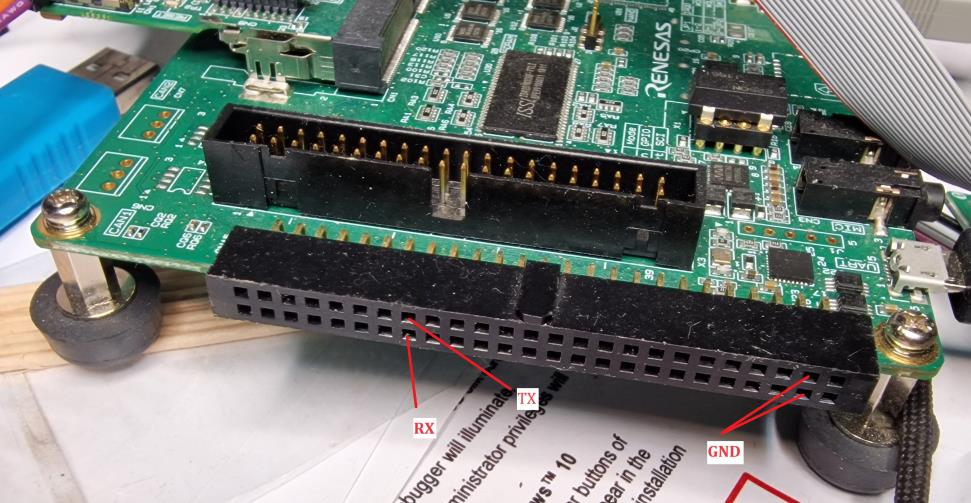
\includegraphics[width=3.75in,height=1.94in]{./media/SCI0_1.jpg}

To test SCI async API via DMA please use the following command:

\begin{lstlisting}
west build -p always -b rz_a2m -S rz-a2m-sci-uart-basic-api-test tests/drivers/uart/uart_basic_api
\end{lstlisting}

\begin{lstlisting}
*** Booting Zephyr OS build zephyr-v3.3.0-10296-g4f74aa9ca078 ***
Running TESTSUITE uart_basic_api
===================================================================
START - test_uart_config_get
This is a configure_get test. PASS - test_uart_config_get in 0.003 seconds
===================================================================
START - test_uart_configure PASS - test_uart_configure in 0.001 seconds
===================================================================
START - test_uart_fifo_fill
This is a FIFO test.
 PASS - test_uart_fifo_fill in 0.501 seconds
===================================================================
START - test_uart_fifo_read
Please send characters to serial console
 PASS - test_uart_fifo_read in 28.315 seconds
===================================================================
START - test_uart_poll_in
Please send characters to serial console
 PASS - test_uart_poll_in in 9.684 seconds
===================================================================
START - test_uart_poll_out
This is a POLL test.
 PASS - test_uart_poll_out in 0.002 seconds
===================================================================
TESTSUITE uart_basic_api succeeded
Running TESTSUITE uart_basic_api_pending
===================================================================
START - test_uart_pending
Please send characters to serial console
d PASS - test_uart_pending in 1.505 seconds
===================================================================
TESTSUITE uart_basic_api_pending succeeded

------ TESTSUITE SUMMARY START ------

SUITE PASS - 100.00% [uart_basic_api]: pass = 6, fail = 0, skip = 0, total = 6 duration = 38.506 seconds
 - PASS - [uart_basic_api.test_uart_config_get] duration = 0.003 seconds
 - PASS - [uart_basic_api.test_uart_configure] duration = 0.001 seconds
 - PASS - [uart_basic_api.test_uart_fifo_fill] duration = 0.501 seconds
 - PASS - [uart_basic_api.test_uart_fifo_read] duration = 28.315 seconds
 - PASS - [uart_basic_api.test_uart_poll_in] duration = 9.684 seconds
 - PASS - [uart_basic_api.test_uart_poll_out] duration = 0.002 seconds

SUITE PASS - 100.00% [uart_basic_api_pending]: pass = 1, fail = 0, skip = 0, total = 1 duration = 1.505 seconds
 - PASS - [uart_basic_api_pending.test_uart_pending] duration = 1.505 seconds

------ TESTSUITE SUMMARY END ------

===================================================================
PROJECT EXECUTION SUCCESSFUL
\end{lstlisting}

Test for async api (using DMA) should be built with following command line
\begin{lstlisting}
west build -p always -b rz_a2m -S rz-a2m-sci-uart-async-api-test tests/drivers/uart/uart_async_api
\end{lstlisting}

After building the image can be started by using command \colorbox{lightgray}{west debug}
and then \colorbox{lightgray}{continue} from the GDB. Please refer to
\hyperref[building-and-flashing]{Building and Flashing} for
the details.

Before running test application, please check pins 15 and 16 on CN15 Connector should be connected.

\begin{lstlisting}
  *** Booting Zephyr OS build v3.5.0-rc2-93-gc5ce8bad57ec ***
  Running TESTSUITE uart_async_chain_read
  ===================================================================
  START - test_chained_read
  SKIP - test_chained_read in 0.001 seconds
  ===================================================================
  TESTSUITE uart_async_chain_read succeeded
  Running TESTSUITE uart_async_chain_write
  ===================================================================
  START - test_chained_write
  PASS - test_chained_write in 0.024 seconds
  ===================================================================
  TESTSUITE uart_async_chain_write succeeded
  Running TESTSUITE uart_async_double_buf
  ===================================================================
  START - test_double_buffer
  SKIP - test_double_buffer in 0.001 seconds
  ===================================================================
  TESTSUITE uart_async_double_buf succeeded
  Running TESTSUITE uart_async_long_buf
  ===================================================================
  START - test_long_buffers
  SKIP - test_long_buffers in 0.001 seconds
  ===================================================================
  TESTSUITE uart_async_long_buf succeeded
  Running TESTSUITE uart_async_multi_rx
  ===================================================================
  START - test_multiple_rx_enable
  SKIP - test_multiple_rx_enable in 0.001 seconds
  ===================================================================
  TESTSUITE uart_async_multi_rx succeeded
  Running TESTSUITE uart_async_read_abort
  ===================================================================
  START - test_read_abort
  PASS - test_read_abort in 1.159 seconds
  ===================================================================
  TESTSUITE uart_async_read_abort succeeded
  Running TESTSUITE uart_async_single_read
  ===================================================================
  START - test_single_read
  PASS - test_single_read in 0.332 seconds
  ===================================================================
  TESTSUITE uart_async_single_read succeeded
  Running TESTSUITE uart_async_timeout
  ===================================================================
  START - test_forever_timeout
  PASS - test_forever_timeout in 3.001 seconds
  ===================================================================
  TESTSUITE uart_async_timeout succeeded
  Running TESTSUITE uart_async_write_abort
  ===================================================================
  START - test_write_abort
  SKIP - test_write_abort in 0.001 seconds
  ===================================================================
  TESTSUITE uart_async_write_abort succeeded
  ------ TESTSUITE SUMMARY START ------
  SUITE SKIP -   0.00% [uart_async_chain_read]: pass = 0, fail = 0, skip = 1, tots
  - SKIP - [uart_async_chain_read.test_chained_read] duration = 0.001 seconds
  SUITE PASS - 100.00% [uart_async_chain_write]: pass = 1, fail = 0, skip = 0, tos
  - PASS - [uart_async_chain_write.test_chained_write] duration = 0.024 seconds
  SUITE SKIP -   0.00% [uart_async_double_buf]: pass = 0, fail = 0, skip = 1, tots
  - SKIP - [uart_async_double_buf.test_double_buffer] duration = 0.001 seconds
  SUITE SKIP -   0.00% [uart_async_long_buf]: pass = 0, fail = 0, skip = 1, totals
  - SKIP - [uart_async_long_buf.test_long_buffers] duration = 0.001 seconds
  SUITE SKIP -   0.00% [uart_async_multi_rx]: pass = 0, fail = 0, skip = 1, totals
  - SKIP - [uart_async_multi_rx.test_multiple_rx_enable] duration = 0.001 seconds
  SUITE PASS - 100.00% [uart_async_read_abort]: pass = 1, fail = 0, skip = 0, tots
  - PASS - [uart_async_read_abort.test_read_abort] duration = 1.159 seconds
  SUITE PASS - 100.00% [uart_async_single_read]: pass = 1, fail = 0, skip = 0, tos
  - PASS - [uart_async_single_read.test_single_read] duration = 0.332 seconds
  SUITE PASS - 100.00% [uart_async_timeout]: pass = 1, fail = 0, skip = 0, total s
  - PASS - [uart_async_timeout.test_forever_timeout] duration = 3.001 seconds
  SUITE SKIP -   0.00% [uart_async_write_abort]: pass = 0, fail = 0, skip = 1, tos
  - SKIP - [uart_async_write_abort.test_write_abort] duration = 0.001 seconds
  ------ TESTSUITE SUMMARY END ------
  ===================================================================
  PROJECT EXECUTION SUCCESSFUL
\end{lstlisting}

Zephyr doesn't have any tests for testing Clock Synchronous mode.

\subsection{Watchdog support}\label{watchdog-support}

Zephyr provides API for the watchdog timer.

This can be checked using the following sample:

\begin{lstlisting}
west build -p always -b rz_a2m samples/drivers/watchdog
\end{lstlisting}

After building the image can be started by using command \colorbox{lightgray}{west debug}
and then \colorbox{lightgray}{continue} from the GDB. Please refer to
\hyperref[building-and-flashing]{Building and Flashing} for the
details.

This sample is part of the Zephyr samples collection. The details about
the test work can be found in the following link:

\url{https://github.com/zephyrproject-rtos/zephyr/blob/main/samples/drivers/watchdog/README.rst}

The result will be the following:

\begin{lstlisting}
*** Booting Zephyr OS build zephyr-v3.4.0-2136-g25fa15563330 ***
Watchdog sample application
Callback in RESET_SOC disabled for this platform
[00:00:00.011,000] <dbg> wdt_rz:
wdt_rz_install_timeout: watchdog@fcfe7000: configuring reset SOC mode
Feeding watchdog 5 times
Feeding watchdog...
Feeding watchdog...
Feeding watchdog...
Feeding watchdog...
Feeding watchdog...
Waiting for reset...
\end{lstlisting}

\subsection{PWM support}\label{pwm-support}

Zephyr supports Pulse Width Modulation (PWM) timer.

This can be tested by running two tests from the box:

\begin{lstlisting}
west build -p always -b rz_a2m tests/drivers/pwm/pwm_api
\end{lstlisting}

After building the image can be started by using command \colorbox{lightgray}{west debug}
and then \colorbox{lightgray}{continue} from the GDB. Please refer to
\hyperref[building-and-flashing]{Building and Flashing} for the
details.

pwm\_api test can be found in the Zephyr source code on the following
path:

\begin{lstlisting}
./tests/drivers/pwm/pwm\_api/
\end{lstlisting}

This test is part of the Zephyr test collection. The details about the
test work can be found in the comment on top of the test source file:

\begin{lstlisting}
./tests/drivers/pwm/pwm_api/src/test_pwm.c
\end{lstlisting}

Console output:

\begin{lstlisting}
*** Booting Zephyr OS build zephyr-v3.4.0-2118-g105a81e409ce ***
Running TESTSUITE pwm_basic
===================================================================
START - test_pwm_cycle
[PWM]: 0, [period]: 64000, [pulse]: 32000
[PWM]: 0, [period]: 64000, [pulse]: 64000
[PWM]: 0, [period]: 64000, [pulse]: 0
PASS - test_pwm_cycle in 3.010 seconds
===================================================================
START - test_pwm_nsec
[PWM]: 0, [period]: 2000000, [pulse]: 1000000
[PWM]: 0, [period]: 2000000, [pulse]: 2000000
[PWM]: 0, [period]: 2000000, [pulse]: 0
PASS - test_pwm_nsec in 3.011 seconds
===================================================================
TESTSUITE pwm_basic succeeded

-------TESTSUITE SUMMARY START -------

SUITE PASS - 100.00% [pwm_basic]: pass = 2, fail =
0, skip = 0, total = 2 duration = 6.021 seconds
- PASS - [pwm_basic.test_pwm_cycle] duration = 3.010 seconds
- PASS - [pwm_basic.test_pwm_nsec] duration = 3.011
seconds

------- TESTSUITE SUMMARY END -------
===================================================================
PROJECT EXECUTION SUCCESSFUL
\end{lstlisting}

For testing both pwm saw-waves and capture mode the next command can be
used (you should connect CN17 pin 24 to CN17 pin 19 for testing):

\begin{lstlisting}
west build -p always -b rz_a2m tests/drivers/pwm/pwm_loopback
\end{lstlisting}

Before running test, please ensure that CN17 pin 24 and CN17 pin 19 are
connected as shown on schema:

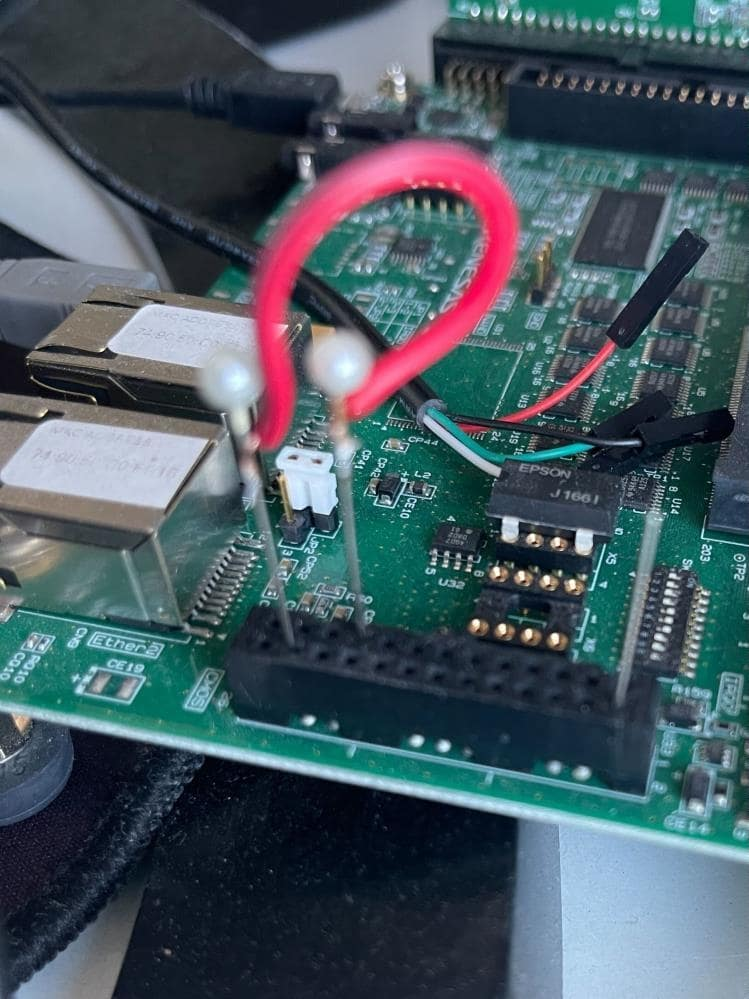
\includegraphics[width=3.75in,height=5in]{./media/image5.jpg}

This test is the part for the Zephyr test collection. It is expected to
be started with the CN17 pins connected (please see above). It generates
a pulse or period from one pin and captures it in the other, then
validates that pulse is the same.

The result will be the following:

\begin{lstlisting}
*** Booting Zephyr OS build zephyr-v3.4.0-2136-g25fa15563330 ***
Running TESTSUITE pwm_loopback
===================================================================
START - test_capture_busy
E: gpt32e1@e8043100: capture started, pls, stop before reconfigutration
E: rza2m_pwm_enable_capture:gpt32e1@e8043100: capture has been
already started
PASS - test_capture_busy in 0.014 seconds
===================================================================
START - test_capture_timeout
W: pwm capture timed out
PASS - test_capture_timeout in 1.002 seconds
===================================================================
START - test_continuous_capture
PASS - test_continuous_capture in 1.076 seconds
===================================================================
START - test_period_capture
Testing PWM capture @ 15000000/100000000 nsec
Testing PWM capture @ 75000/100000 usec
PASS - test_period_capture in 0.313 seconds
===================================================================
START - test_period_capture_inverted
Testing PWM capture @ 15000000/100000000 nsec
Testing PWM capture @ 75000/100000 usec
PASS - test_period_capture_inverted in 0.388 seconds
===================================================================
START - test_pulse_and_period_capture
Testing PWM capture @ 15000000/100000000 nsec
Testing PWM capture @ 75000/100000 usec
PASS - test_pulse_and_period_capture in 0.387 seconds
===================================================================
START - test_pulse_capture
Testing PWM capture @ 15000000/100000000 nsec
Testing PWM capture @ 75000/100000 usec
PASS - test_pulse_capture in 0.263 seconds
===================================================================
START - test_pulse_capture_inverted
Testing PWM capture @ 15000000/100000000 nsec
Testing PWM capture @ 75000/100000 usec
PASS - test_pulse_capture_inverted in 0.288 seconds
===================================================================

TESTSUITE pwm_loopback succeeded

------- TESTSUITE SUMMARY START -------

SUITE PASS - 100.00% [pwm_loopback]: pass = 8, fail = 0, skip = 0,
total = 8 duration = 3.731 seconds
- PASS - [pwm_loopback.test_capture_busy] duration = 0.014
seconds
- PASS - [pwm_loopback.test_capture_timeout] duration = 1.002
seconds
- PASS - [pwm_loopback.test_continuous_capture] duration = 1.076
seconds
- PASS - [pwm_loopback.test_period_capture] duration = 0.313
seconds
- PASS - [pwm_loopback.test_period_capture_inverted] duration =
0.388 seconds
- PASS - [pwm_loopback.test_pulse_and_period_capture] duration
= 0.387 seconds
- PASS - [pwm_loopback.test_pulse_capture] duration = 0.263
seconds
- PASS - [pwm_loopback.test_pulse_capture_inverted] duration =
0.288 seconds

------- TESTSUITE SUMMARY END -------

===================================================================

PROJECT EXECUTION SUCCESSFUL
\end{lstlisting}

\subsection{I2C support}\label{i2c}

Zephyr supports interface for I2C (Inter-Integrated Circuit) is a
commonly used two-signal shared peripheral interface bus. Many
system-on-chip solutions provide controllers that communicate on an I2C
bus. Devices on the bus can operate in two roles: as a \colorbox{lightgray}{controller}
that initiates transactions and controls the clock, or as a \colorbox{lightgray}{target}
that responds to transaction commands. An I2C controller on a given SoC
will generally support the controller role, and some will also support
the target mode. Zephyr has API for both roles.

For the testing purposes BME280 sensor was connected to the board and
the following test was started:

\begin{lstlisting}
west build -p always -b rz_a2m samples/sensor/bme280
\end{lstlisting}

After building the image can be started by using command \colorbox{lightgray}{west debug}
and then \colorbox{lightgray}{continue} from the GDB. Please refer to
\hyperref[building-and-flashing]{Building and Flashing} for the
details.

This test is part of the Zephyr test collection. The details about the
test work can be found on the following link:
\url{https://docs.zephyrproject.org/latest/samples/sensor/bme280/README.html}

BME280 sensor we used looks like this:

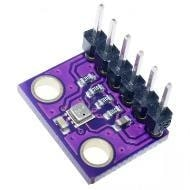
\includegraphics[width=0.9532in,height=0.9532in]{./media/sensor.jpg}

Bosch BME280 sensor website:
\href{https://www.bosch-sensortec.com/products/environmental-sensors/humidity-sensors-bme280/}{Bosch Sensor Link}

Sensor can be bought:
\href{https://www.ebay.com/itm/364383183367?hash=item54d6ee2207:g:9nEAAOSw4cpkxb8e&amdata=enc%3AAQAIAAAA4CNZsveLKwB%2Bbtxwddq1XA6AG7ZzLUZUtkEJhofNOcOAZjNwrE0ntieLQd5z8eMQSMN4aEAFGeL9B0uKgDHIB5ddwS%2Fi527%2BUBISab8tuIGQ8kBnJHzsWjBE694%2BuPxyY3NLa1RkA3foa27rLBqN1YVo03DFl%2B2%2BNc1wHeuZNNm0jSITv1Aso5b2eog66imoO2sq3R6BcKmTUTOX7s97n0S8hSnJw1F0QVlssPYZjHj%2FX4oZGFYYy5uiIgy5LghN4WszDLbwRhgW4WY%2B61Xdgdm91qSggfJF3wPw05%2BA2AAt%7Ctkp%3ABFBMtKColdxi}{Bosch Sensor Product}

The connection schema on Subboard CN17 connector is the following:

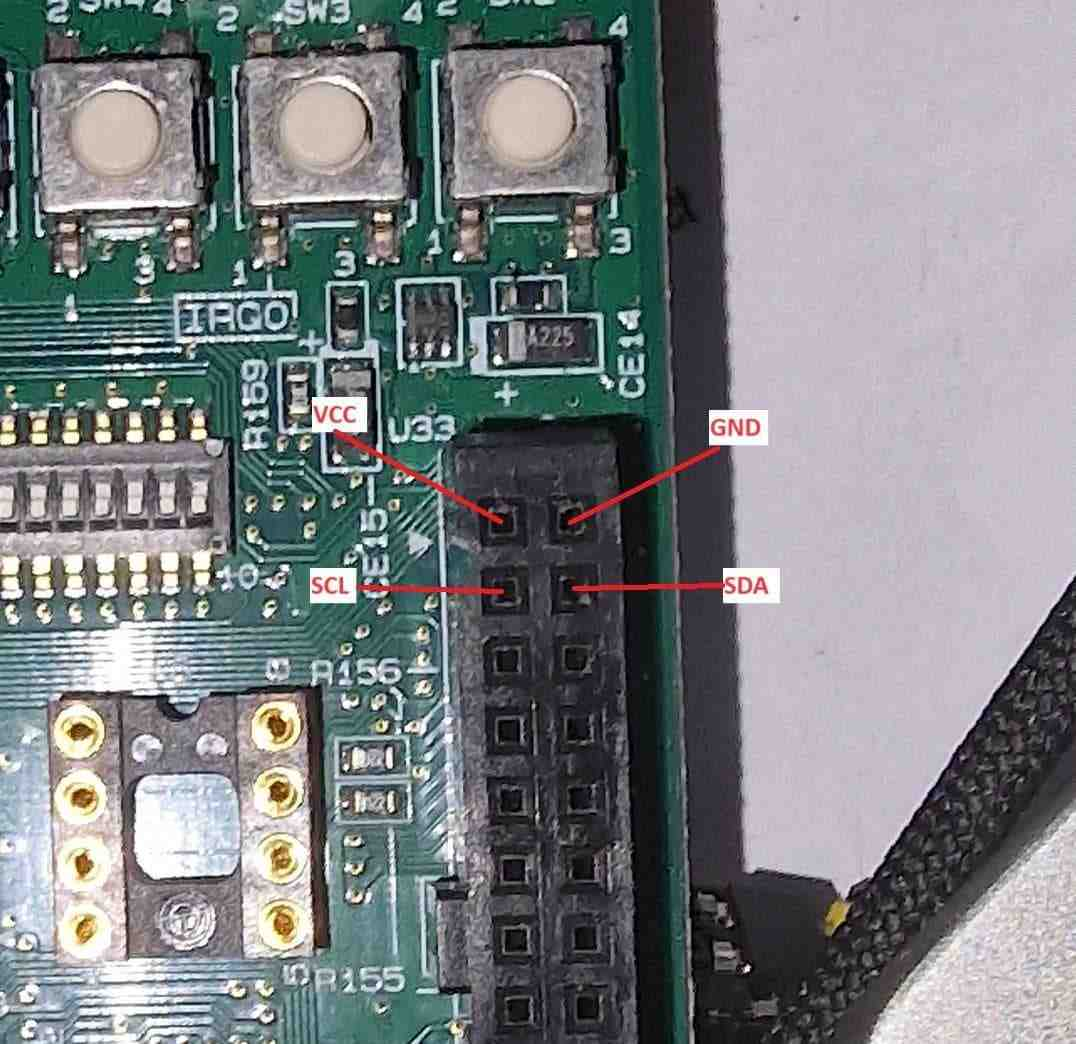
\includegraphics[width=5in,height=4.85417in]{./media/uart_conn.jpg}

The result is the following:

\begin{lstlisting}
[00:00:00.002,000] <dbg> BME280:
bme280_chip_init: ID OK
[00:00:00.046,000] <dbg> BME280:
bme280_chip_init: "bme280@76" OK
*** Booting Zephyr OS build zephyr-v3.3.0-7308-g33a43667b550 ***
Found device "bme280@76", getting sensor data
temp: 28.250000; press: 100.356968; humidity: 37.498046
temp: 28.250000; press: 100.355968; humidity: 37.427734
temp: 28.260000; press: 100.355085; humidity: 37.381835
temp: 28.260000; press: 100.354585; humidity: 37.334960
temp: 28.260000; press: 100.355093; humidity: 37.277343
temp: 28.260000; press: 100.354671; humidity: 37.252929
temp: 28.260000; press: 100.355257; humidity: 37.500000
temp: 28.270000; press: 100.355472; humidity: 40.737304
temp: 28.280000; press: 100.355101; humidity: 42.736328
temp: 28.440000; press: 100.353152; humidity: 54.832031
temp: 28.790000; press: 100.353847; humidity: 68.174804
temp: 28.960000; press: 100.354117; humidity: 69.546875
temp: 29.170000; press: 100.353585; humidity: 72.966796
temp: 29.480000; press: 100.354390; humidity: 77.227539
temp: 29.670000; press: 100.356492; humidity: 77.467773
temp: 29.870000; press: 100.356449; humidity: 79.854492
temp: 30.100000; press: 100.357484; humidity: 81.495117
temp: 30.230000; press: 100.357480; humidity: 79.442382
temp: 30.270000; press: 100.357996; humidity: 75.188476
temp: 30.280000; press: 100.358199; humidity: 68.515625
temp: 30.260000; press: 100.359214; humidity: 60.868164
temp: 30.220000; press: 100.358734; humidity: 55.585937
\end{lstlisting}

If you want to test the parallel operation of sensors on the same I2C bus,
you can use the following test:

\begin{lstlisting}
west build -p always -b rz_a2m samples/sensor/ina219_2sensors
\end{lstlisting}

After building the image can be started by using command \colorbox{lightgray}{west debug}
and then \colorbox{lightgray}{continue} from the GDB. Please refer to
\hyperref[building-and-flashing]{Building and Flashing} for the
details.

For this test you will need 2 INA219 sensor modules. Here's what it looks like:

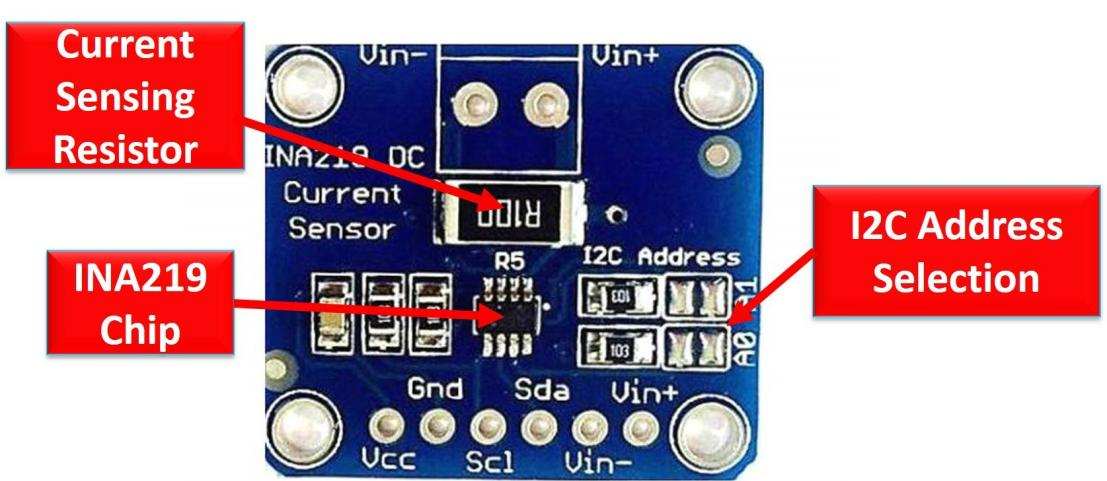
\includegraphics[width=5in]{./media/INA219_Module.jpg}

TI INA219 sensor website:
\href{https://www.ti.com/product/INA219}{TI INA219 Page Link}

Module can be bought:
\href{https://www.ebay.com/itm/266045143022?hash=item3df186b7ee:g:WgcAAOSwV8hjndFy&amdata=enc%3AAQAIAAAA4G3Cdgx8lqumNzR84HG5F%2FRa3SAIkQfAsqucnJhd9VktjVIIbxEVn%2FcBUvOpdiEI2lvKpHxeGi%2Fhtyj10XWYiVcdqCpPFvs6ArJXy7il4Fgk0JaWghpQnfz1%2FUQwZ6J6Ne1k02G5gtKKsbf3miD9MQNgCii%2B4DnnAMjsACTISV7OSLZnCBNTBwapu4U3mQZgVKeGFjfmdjgIgRbd20NgqymaY5VOyzliPqPc2Wku7kS%2BGndGjUVem3tT7BXr4iEJeMlbZgd1ZdHncruw6ni%2F2l1071%2BoF%2FUx18XerDyZCok%2B%7Ctkp%3ABk9SR_7ws7ztYg}{INA219 Module Product}

The connection schema to Subboard CN17 connector is the following:

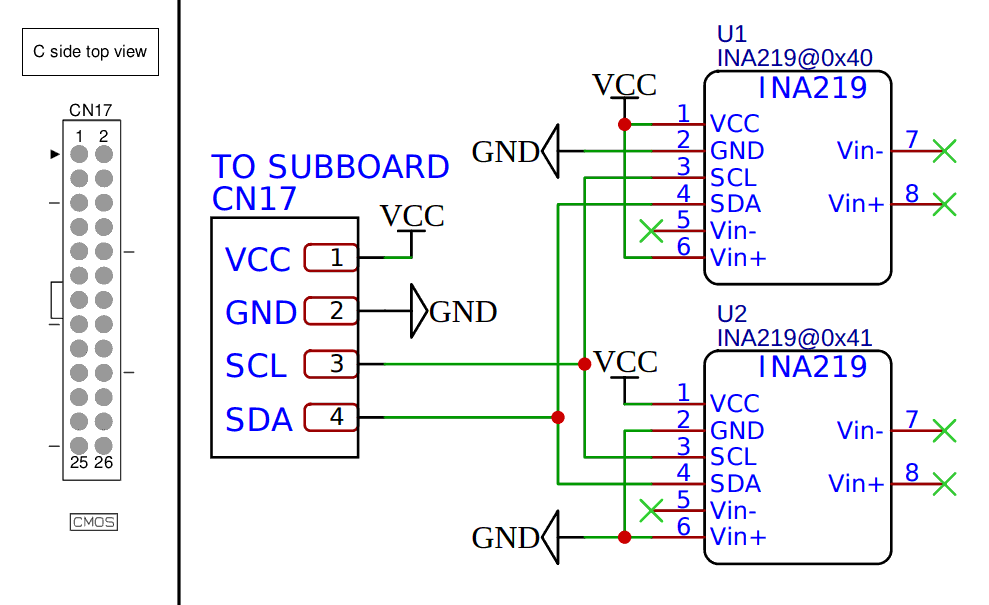
\includegraphics[width=5in]{./media/INA219_connection.png}

Please note that before connecting you need to change the U2 module address to 0x41
by soldering jumper A0 on the module. The U1 address remains unchanged (0x40).
More information about changing the address is described here:
\href{https://whatibroke.com/2019/08/10/change-i2c-address-of-ina219/}{INA219 I2C Address Change}

As a result, you will receive the following output in the console:

\begin{lstlisting}
*** Booting Zephyr OS build v3.5.0-rc2-75-g6576263fd108 ***
ID      Bus[V]  Pow[W]  Curr[A]
0       3       0       0
1       0       0       0
0       3       0       0
1       0       0       0
0       3       0       0
1       0       0       0
0       3       0       0
1       0       0       0
0       3       0       0
1       0       0       0
0       3       0       0
1       0       0       0
0       3       0       0
\end{lstlisting}

This means that the sensor with ID=0 (U1) has a voltage of about 3V at the VIN+ input,
and the sensor with ID=1 (U2) has 0V at the VIN+ input. We output to the console only the
integer part of the values received from the sensors in order to reduce the delays
introduced into each thread by the output function.

\subsubsection{I2C Target support}\label{i2c-target-support}

Zephyr supports \colorbox{lightgray}{target (slave)} mode for the I2C bus, as well as the
so-called \colorbox{lightgray}{dual role mode}, when one bus can simultaneously
be both a master and a slave. To test these modes, you can use the basic test:

\begin{lstlisting}
west build -p always -b rz_a2m tests/drivers/i2c/i2c_target_api/
\end{lstlisting}

After building the image can be started by using command \colorbox{lightgray}{west debug}
and then \colorbox{lightgray}{continue} from the GDB. Please refer to
\hyperref[building-and-flashing]{Building and Flashing} for the
details.

This test emulates the operation of I2C EEPROM memory on the i2c2 bus in slave mode
and attempts to perform EEPROM read/write operations using the i2c3 bus in master mode.
After this, the roles of the i2c2 and i2c3 buses change and the test is repeated.
For this test to work, you must first connect the i2c2 and i2c3 buses to each other
according to the diagram:

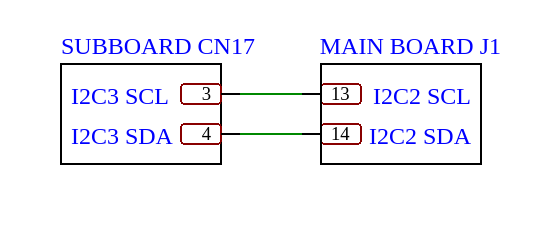
\includegraphics[width=4in]{./media/I2C_Target_connection.png}

The test result is following:

\begin{lstlisting}
*** Booting Zephyr OS build v3.5.0-rc2-97-gd699393f4c85 ***
Running TESTSUITE i2c_eeprom_target
===================================================================
START - test_eeprom_target
Found EEPROM 0 on I2C bus device i2c@e803a800 at addr 54
Found EEPROM 1 on I2C bus device i2c@e803ac00 at addr 56
Testing dual-role
Testing full read: Master: i2c@e803ac00, address: 0x54
Testing full read: Master: i2c@e803a800, address: 0x56
Testing partial read. Master: i2c@e803ac00, address: 0x54, off=0
Testing partial read. Master: i2c@e803a800, address: 0x56, off=0
Testing partial read. Master: i2c@e803ac00, address: 0x54, off=1
Testing partial read. Master: i2c@e803a800, address: 0x56, off=1
Testing partial read. Master: i2c@e803ac00, address: 0x54, off=2
Testing partial read. Master: i2c@e803a800, address: 0x56, off=2
Testing partial read. Master: i2c@e803ac00, address: 0x54, off=3
Testing partial read. Master: i2c@e803a800, address: 0x56, off=3
Testing partial read. Master: i2c@e803ac00, address: 0x54, off=4
Testing partial read. Master: i2c@e803a800, address: 0x56, off=4
Testing partial read. Master: i2c@e803ac00, address: 0x54, off=5
Testing partial read. Master: i2c@e803a800, address: 0x56, off=5
Testing partial read. Master: i2c@e803ac00, address: 0x54, off=6
Testing partial read. Master: i2c@e803a800, address: 0x56, off=6
Testing partial read. Master: i2c@e803ac00, address: 0x54, off=7
Testing partial read. Master: i2c@e803a800, address: 0x56, off=7
Testing partial read. Master: i2c@e803ac00, address: 0x54, off=8
Testing partial read. Master: i2c@e803a800, address: 0x56, off=8
Testing partial read. Master: i2c@e803ac00, address: 0x54, off=9
Testing partial read. Master: i2c@e803a800, address: 0x56, off=9
Testing partial read. Master: i2c@e803ac00, address: 0x54, off=10
Testing partial read. Master: i2c@e803a800, address: 0x56, off=10
Testing partial read. Master: i2c@e803ac00, address: 0x54, off=11
Testing partial read. Master: i2c@e803a800, address: 0x56, off=11
Testing partial read. Master: i2c@e803ac00, address: 0x54, off=12
Testing partial read. Master: i2c@e803a800, address: 0x56, off=12
Testing partial read. Master: i2c@e803ac00, address: 0x54, off=13
Testing partial read. Master: i2c@e803a800, address: 0x56, off=13
Testing partial read. Master: i2c@e803ac00, address: 0x54, off=14
Testing partial read. Master: i2c@e803a800, address: 0x56, off=14
Testing partial read. Master: i2c@e803ac00, address: 0x54, off=15
Testing partial read. Master: i2c@e803a800, address: 0x56, off=15
Testing partial read. Master: i2c@e803ac00, address: 0x54, off=16
Testing partial read. Master: i2c@e803a800, address: 0x56, off=16
Testing partial read. Master: i2c@e803ac00, address: 0x54, off=17
Testing partial read. Master: i2c@e803a800, address: 0x56, off=17
Testing partial read. Master: i2c@e803ac00, address: 0x54, off=18
Testing partial read. Master: i2c@e803a800, address: 0x56, off=18
Testing program. Master: i2c@e803ac00, address: 0x54, off=0
Testing program. Master: i2c@e803a800, address: 0x56, off=0
Testing program. Master: i2c@e803ac00, address: 0x54, off=1
Testing program. Master: i2c@e803a800, address: 0x56, off=1
Testing program. Master: i2c@e803ac00, address: 0x54, off=2
Testing program. Master: i2c@e803a800, address: 0x56, off=2
Testing program. Master: i2c@e803ac00, address: 0x54, off=3
Testing program. Master: i2c@e803a800, address: 0x56, off=3
Testing program. Master: i2c@e803ac00, address: 0x54, off=4
Testing program. Master: i2c@e803a800, address: 0x56, off=4
Testing program. Master: i2c@e803ac00, address: 0x54, off=5
Testing program. Master: i2c@e803a800, address: 0x56, off=5
Testing program. Master: i2c@e803ac00, address: 0x54, off=6
Testing program. Master: i2c@e803a800, address: 0x56, off=6
Testing program. Master: i2c@e803ac00, address: 0x54, off=7
Testing program. Master: i2c@e803a800, address: 0x56, off=7
Testing program. Master: i2c@e803ac00, address: 0x54, off=8
Testing program. Master: i2c@e803a800, address: 0x56, off=8
Testing program. Master: i2c@e803ac00, address: 0x54, off=9
Testing program. Master: i2c@e803a800, address: 0x56, off=9
Testing program. Master: i2c@e803ac00, address: 0x54, off=10
Testing program. Master: i2c@e803a800, address: 0x56, off=10
Testing program. Master: i2c@e803ac00, address: 0x54, off=11
Testing program. Master: i2c@e803a800, address: 0x56, off=11
Testing program. Master: i2c@e803ac00, address: 0x54, off=12
Testing program. Master: i2c@e803a800, address: 0x56, off=12
Testing program. Master: i2c@e803ac00, address: 0x54, off=13
Testing program. Master: i2c@e803a800, address: 0x56, off=13
Testing program. Master: i2c@e803ac00, address: 0x54, off=14
Testing program. Master: i2c@e803a800, address: 0x56, off=14
Testing program. Master: i2c@e803ac00, address: 0x54, off=15
Testing program. Master: i2c@e803a800, address: 0x56, off=15
Testing program. Master: i2c@e803ac00, address: 0x54, off=16
Testing program. Master: i2c@e803a800, address: 0x56, off=16
Testing program. Master: i2c@e803ac00, address: 0x54, off=17
Testing program. Master: i2c@e803a800, address: 0x56, off=17
Testing program. Master: i2c@e803ac00, address: 0x54, off=18
Testing program. Master: i2c@e803a800, address: 0x56, off=18
PASS - test_eeprom_target in 0.719 seconds
===================================================================
TESTSUITE i2c_eeprom_target succeeded

------ TESTSUITE SUMMARY START ------

SUITE PASS - 100.00% [i2c_eeprom_target]: pass = 1, fail = 0, skip = 0, total =s
- PASS - [i2c_eeprom_target.test_eeprom_target] duration = 0.719 seconds

------ TESTSUITE SUMMARY END ------

===================================================================
PROJECT EXECUTION SUCCESSFUL
\end{lstlisting}

\subsection{DMA}\label{dma}

Zephyr also provides an interface for the DMA controller.

This support can be tested using the following commands:

\begin{lstlisting}
west build -p always -b rz_a2m tests/drivers/dma/chan_blen_transfer
west build -p always -b rz_a2m tests/drivers/dma/loop_transfer
west build -p always -b rz_a2m tests/drivers/dma/scatter_gather
\end{lstlisting}

After building the image can be started by using command \colorbox{lightgray}{west debug}
and then \colorbox{lightgray}{continue} from the GDB. Please refer to
\hyperref[building-and-flashing]{Building and Flashing} for the
details.

The tests provided support only MEMORY\_TO\_MEMORY communication.

chan\_blen\_transfer test can be found in the Zephyr source code on the
following path:

\begin{lstlisting}
./tests/drivers/dma/chan_blen_transfer/
\end{lstlisting}

This test is part of the Zephyr test collection. The details about the
test work can be found in the comment on top of the test source file:
\begin{lstlisting}
./tests/drivers/dma/chan_blen_transfer/src/test_dma.c
\end{lstlisting}

Output example for clan\_blen\_transfer:

\begin{lstlisting}
*** Booting Zephyr OS build zephyr-v3.4.0-2118-ge546b2e5fcac ***
Running TESTSUITE dma_m2m
===================================================================
START - test_test_dma0_m2m_chan0_burst16
Preparing DMA Controller: Name=dma@e8226000, Chan_ID=0, BURST_LEN=2
Starting the transfer
DMA transfer done
It is harder to be kind than to be wise........
PASS - test_test_dma0_m2m_chan0_burst16 in 2.012 seconds
===================================================================
START - test_test_dma0_m2m_chan0_burst8
Preparing DMA Controller: Name=dma@e8226000, Chan_ID=0, BURST_LEN=1
Starting the transfer
DMA transfer done
It is harder to be kind than to be wise........
PASS - test_test_dma0_m2m_chan0_burst8 in 2.012 seconds
===================================================================
START - test_test_dma0_m2m_chan1_burst16
Preparing DMA Controller: Name=dma@e8226000, Chan_ID=1, BURST_LEN=2
Starting the transfer
DMA transfer done
It is harder to be kind than to be wise........
PASS - test_test_dma0_m2m_chan1_burst16 in 2.012 seconds
===================================================================
START - test_test_dma0_m2m_chan1_burst8
Preparing DMA Controller: Name=dma@e8226000, Chan_ID=1, BURST_LEN=1
Starting the transfer
DMA transfer done
It is harder to be kind than to be wise........
PASS - test_test_dma0_m2m_chan1_burst8 in 2.012 seconds
===================================================================
TESTSUITE dma_m2m succeeded

------- TESTSUITE SUMMARY START -------

SUITE PASS - 100.00% [dma_m2m]: pass = 4, fail = 0, skip = 0,
total = 4 duration = 8.048 seconds
- PASS - [dma_m2m.test_test_dma0_m2m_chan0_burst16] duration =
2.012 seconds
- PASS - [dma_m2m.test_test_dma0_m2m_chan0_burst8] duration =
2.012 seconds
- PASS - [dma_m2m.test_test_dma0_m2m_chan1_burst16] duration =
2.012 seconds
- PASS - [dma_m2m.test_test_dma0_m2m_chan1_burst8] duration =
2.012 seconds

------- TESTSUITE SUMMARY END -------
===================================================================

PROJECT EXECUTION SUCCESSFUL
\end{lstlisting}

loop\_transfer test can be found in the Zephyr source code on the
following path:

\begin{lstlisting}
./tests/drivers/dma/loop_transfer/
\end{lstlisting}

This test is part of the Zephyr test collection. The details about the
test work can be found in the comment on top of the test source file:
\begin{lstlisting}
./tests/drivers/dma/loop_transfer/src/test_dma_loop.c
\end{lstlisting}

Test loop\_transfer output:

\begin{lstlisting}
*** Booting Zephyr OS build zephyr-v3.4.0-2146-gb8d969dcbb21 ***

Running TESTSUITE dma_m2m_loop
===================================================================
START - test_test_dma0_m2m_loop
DMA memory to memory transfer started
Preparing DMA Controller: dma@e8226000
Starting the transfer on channel 0 and waiting for 1 second
Each RX buffer should contain the full TX buffer string.
RX data Loop 0
RX data Loop 1
RX data Loop 2
RX data Loop 3
Finished DMA: dma@e8226000
PASS - test_test_dma0_m2m_loop in 0.281 seconds
===================================================================
START - test_test_dma0_m2m_loop_repeated_start_stop
DMA memory to memory transfer started
Preparing DMA Controller
Starting the transfer on channel 1 and waiting for 1 second
Each RX buffer should contain the full TX buffer string.
RX data Loop 0
RX data Loop 1
RX data Loop 2
RX data Loop 3
Finished: DMA
PASS - test_test_dma0_m2m_loop_repeated_start_stop in 0.278
seconds
===================================================================
START - test_test_dma0_m2m_loop_suspend_resume
DMA memory to memory transfer started
Preparing DMA Controller: dma@e8226000
Starting the transfer on channel 2 and waiting for 1 second
suspended after 0 transfers occurred
resuming after 0 transfers occurred
Resumed transfers
Transfer count 4
Each RX buffer should contain the full TX buffer string.
RX data Loop 0
RX data Loop 1
RX data Loop 2
RX data Loop 3
Finished DMA: dma@e8226000
PASS - test_test_dma0_m2m_loop_suspend_resume in 0.540 seconds
===================================================================
TESTSUITE dma_m2m_loop succeeded

------- TESTSUITE SUMMARY START -------

SUITE PASS - 100.00% [dma_m2m_loop]: pass = 3, fail = 0, skip =
0, total = 3 duration = 1.099 seconds
- PASS - [dma_m2m_loop.test_test_dma0_m2m_loop] duration =
0.281 seconds
- PASS -
[dma_m2m_loop.test_test_dma0_m2m_loop_repeated_start_stop]
duration = 0.278 seconds
- PASS -
[dma_m2m_loop.test_test_dma0_m2m_loop_suspend_resume]
duration = 0.540 seconds

------- TESTSUITE SUMMARY END -------
===================================================================

PROJECT EXECUTION SUCCESSFUL
\end{lstlisting}

scatter\_gather test can be found in the Zephyr source code on the
following path:
\begin{lstlisting}
./tests/drivers/dma/scatter_gather/
\end{lstlisting}

This test is part of the Zephyr test collection. The details about the
test work can be found in the comment on top of the test source file:
\begin{lstlisting}
./tests/drivers/dma/scatter_gather/src/test_dma_sg.c
\end{lstlisting}

Test execution output:

\begin{lstlisting}
*** Booting Zephyr OS build zephyr-v3.4.0-2146-gb8d969dcbb21 ***

Running TESTSUITE dma_m2m_sg
===================================================================
START - test_dma_m2m_sg
DMA memory to memory transfer started
Preparing DMA Controller
dma block 0 block_size 8192, source addr 80034000, dest addr 80036000
set next block pointer to 0x80054244
dma block 1 block_size 8192, source addr 80034000, dest addr 80038000
set next block pointer to 0x80054264
dma block 2 block_size 8192, source addr 80034000, dest addr 8003a000
set next block pointer to 0x80054284
dma block 3 block_size 8192, source addr 80034000, dest addr 8003c000
Configuring the scatter-gather transfer on channel 0
Starting the transfer on channel 0 and waiting completion
giving xfer_sem
Verify RX buffer should contain the full TX buffer string.
rx_data[0]
rx_data[1]
rx_data[2]
rx_data[3]
Finished: DMA Scatter-Gather
PASS - test_dma_m2m_sg in 0.071 seconds
===================================================================
TESTSUITE dma_m2m_sg succeeded

------- TESTSUITE SUMMARY START -------

SUITE PASS - 100.00% [dma_m2m_sg]: pass = 1, fail = 0, skip = 0,
total = 1 duration = 0.071 seconds
- PASS - [dma_m2m_sg.test_dma_m2m_sg] duration = 0.071 seconds

------- TESTSUITE SUMMARY END -------
===================================================================

PROJECT EXECUTION SUCCESSFUL
\end{lstlisting}

\subsection{RTC}\label{rtc}

An RTC is a low power device which tracks time using broken-down time.
It should not be confused with low-power counters which sometimes share
the same name, acronym, or both.

RTCs are usually optimized for low energy consumption and are usually
kept running even when the system is in a low power state.

RTCs usually contain one or more alarms which can be configured to
trigger at a given time. These alarms are commonly used to wake up the
system from a low power state.

This can be tested using the following command:

\begin{lstlisting}
west build -p always -b rz_a2m tests/drivers/rtc/rtc_api
\end{lstlisting}

This test is part of the Zephyr test collection. The details about the
test work can be found on the link:

\url{https://docs.zephyrproject.org/latest/hardware/peripherals/rtc.html\#rtc-device-driver-test-suite}

After building the image can be started by using command \colorbox{lightgray}{west debug}
and then \colorbox{lightgray}{continue} from the GDB. Please refer to
\hyperref[building-and-flashing]{Building and Flashing} for the
details.

Sample of tests output:

\begin{lstlisting}
*** Booting Zephyr OS build zephyr-v3.4.0-2136-g25fa15563330 ***

Running TESTSUITE rtc_api
===================================================================
START - test_alarm
PASS - test_alarm in 26.096 seconds
===================================================================
START - test_alarm_callback
PASS - test_alarm_callback in 26.128 seconds
===================================================================
START - test_set_get_calibration
Calibrate (set,get): 1, 1
Calibrate (set,get): -1, 1
E: rtc@fcff1000: currently support calibration values from the next
range [-6;6] Hz
E: rtc@fcff1000: currently support calibration values from the next
range [-6;6] Hz
PASS - test_set_get_calibration in 0.020 seconds
===================================================================
START - test_set_get_time
PASS - test_set_get_time in 0.001 seconds
===================================================================
START - test_time_counting
PASS - test_time_counting in 10.003 seconds
===================================================================
START - test_update_callback
PASS - test_update_callback in 15.001 seconds
===================================================================

TESTSUITE rtc_api succeeded

------- TESTSUITE SUMMARY START -------

SUITE PASS - 100.00% [rtc_api]: pass = 6, fail = 0, skip = 0,
total = 6 duration = 77.249 seconds
- PASS - [rtc_api.test_alarm] duration = 26.096 seconds
- PASS - [rtc_api.test_alarm_callback] duration = 26.128 seconds
- PASS - [rtc_api.test_set_get_calibration] duration = 0.020
seconds
- PASS - [rtc_api.test_set_get_time] duration = 0.001 seconds
- PASS - [rtc_api.test_time_counting] duration = 10.003 seconds
- PASS - [rtc_api.test_update_callback] duration = 15.001 seconds

------- TESTSUITE SUMMARY END -------
===================================================================

PROJECT EXECUTION SUCCESSFUL
\end{lstlisting}

\subsection{OSTM}\label{ostm}

The OSTM is a multi-channel 32-bit timer/counter with fixed clock source
that can operate in either interval count down timer or free-running
compare match mode.

Zephyr has the following test:

\begin{lstlisting}
west build -p always -b rz_a2m tests/kernel/tickless/tickless_concept/
\end{lstlisting}

After building the image can be started by using command \colorbox{lightgray}{west debug}
and then \colorbox{lightgray}{continue} from the GDB. Please refer to
\hyperref[building-and-flashing]{Building and Flashing} for the
details.

This test is part of the Zephyr test collection. Validates work with and
without tickless idle and verify tickless functionality with a time
slice.

The result is the following:

\begin{lstlisting}
*** Booting Zephyr OS build zephyr-v3.4.0-2136-g25fa15563330 ***

Running TESTSUITE tickless_concept
===================================================================
START - test_tickless_slice
elapsed slice 110, expected: <100, 110>
elapsed slice 100, expected: <100, 110>
elapsed slice 100, expected: <100, 110>
elapsed slice 100, expected: <100, 110>
PASS - test_tickless_slice in 0.606 seconds
===================================================================
START - test_tickless_sysclock
time 640, 850
time 860, 1060
PASS - test_tickless_sysclock in 0.426 seconds
===================================================================

TESTSUITE tickless_concept succeeded

------- TESTSUITE SUMMARY START -------

SUITE PASS - 100.00% [tickless_concept]: pass = 2, fail = 0, skip
= 0, total = 2 duration = 1.032 seconds
- PASS - [tickless_concept.test_tickless_slice] duration = 0.606
seconds
- PASS - [tickless_concept.test_tickless_sysclock] duration =
0.426 seconds

------- TESTSUITE SUMMARY END -------
===================================================================

PROJECT EXECUTION SUCCESSFUL
\end{lstlisting}

Also, you can run:

\begin{lstlisting}
west build -p always -b rz_a2m tests/kernel/sleep/
\end{lstlisting}

\subsection{BSC}\label{bsc}

The bus state controller outputs control signals for various types of
memory and external devices that are connected to the external address
space. The functions of this module enable this LSI to connect directly
with SRAM, SDRAM, and other memory storage devices, and external
devices.

The following test can be run:

\begin{lstlisting}
west build -p always -b rz_a2m tests/drivers/bsc/rz_a2m
\end{lstlisting}

After building the image can be started by using command \colorbox{lightgray}{west debug}
and then \colorbox{lightgray}{continue} from the GDB. Please refer to
\hyperref[building-and-flashing]{Building and Flashing} for the
details.

This test is intended to verify SDRAM connection to the CPU board. To
perform this operation the board should be reconfigured as mentioned in
NOTE below. This test initializes SDRAM from the SUBBOARD, maps it to
the Zephyr address space and verifies that this address space is
accessible from the code.

NOTE: When SDRAM is connected\\
You must change switch SW6\_1 to "ON" to enable SDRAM bus\\
You must also change switch SW6\_3 to "ON'' to detach USB-serial from
SDRAM bus\\
You must also change switch SW6\_4 to "OFF" to enable SCIF-2 on CN17

SCIF4 connection (CN5 miniUSB attached to the PC) see Diagram on
\hyperref[board-initial-configuration]{Board initial configuration}
details, doesn't work in this mode. So SCIF2 should be connected.

To connect SCIF2 to the PC the following adapter should be used:

\href{https://www.ebay.com/itm/374576049950?hash=item573678ef1e:g:v1sAAOSwx7pkGapp&amdata=enc%3AAQAIAAAA8MQ4P8oojMoR6H4TwJkrlrD0d39kQ7hfOOSnDeCt%2Bp3hjsAZsig8OM8eNojvjmkFV5rzU3w89k8DUQRijARt5vJV6nEF8vslmPLoG%2F9rEO4iy%2BYYnA8w3IR8Vqh7fuWcA2zkr1483%2FK4b1ianYJT%2BRnJkO5w%2FmHajRHkP8Et5fxsovnGXJH58bJCnbJTqB5lLAcFF%2FmVTEn86GlCnc0GgqxhcNJVjpJRhxwsb49LQajClAH%2F%2BU01LcJBLxqCBABTiPj0GPFBi%2BjUOX3uDEhu1qCSVopHX%2BfdeM3TS2k9qYZbvkRViqIr%2FZfGa5AprKoH9w%3D%3D%7Ctkp%3ABFBM1rL9heNi}{SCIF adapter Product Page}

It looks like this:


\includegraphics[width=3.03125in,height=3.16708in]{./media/cable.jpg}

SCIF2 can be connected to the following pins on CN17 connector:
GND -- pin 2, RXD -- pin 10 and TXD -- pin 9. The USB should be attached
to the Spare USB port in your PC.

After testing, please switch the SW6 to the original state and reconnect
CN5 to your PC.

Test preparation steps:

\begin{enumerate}
\def\labelenumi{\arabic{enumi})}
\item
  Turn off the board.
\item
  Set SW6\_1 to "ON", SW6\_3 to "ON'' and SW6\_4 to "OFF".
\item
  Connect usb cable to CN17 pins 2, 9 and 10 as shown on schema:
\end{enumerate}

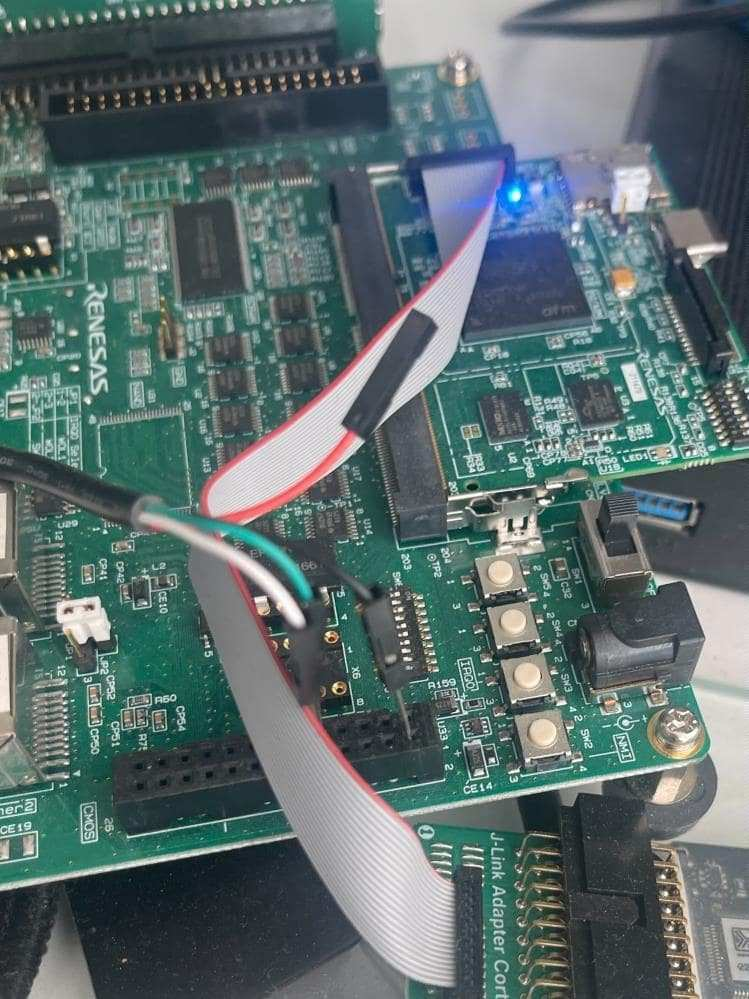
\includegraphics[width=3.75in,height=5in]{./media/scif2_conn.jpg}

\begin{enumerate}
\def\labelenumi{\arabic{enumi})}
\setcounter{enumi}{3}
\item
  Connect USB cable (connected to CN17 on the previous step) to your PC
  and attach it to the PC.
\item
  Use minicom to connect to the Serial Console. Please note that
  /dev/ttyX different so please use steps from Section 4. Board Initial
  Configuration to find correct /dev/ttyX device.
\item
  Turn on the board and perform test.
\item
  Don't forget to switch back the board to the initial state.
\end{enumerate}

The result will be the following.

\begin{lstlisting}
*** Booting Zephyr OS build zephyr-v3.4.0-2121-gffc8faec07c9 ***

Running TESTSUITE bsc_rza2_suite
===================================================================
START - test_mem_set
PASS - test_mem_set in 0.001 seconds
===================================================================

TESTSUITE bsc_rza2_suite succeeded

------- TESTSUITE SUMMARY START -------

SUITE PASS - 100.00% [bsc_rza2_suite]: pass = 1, fail = 0, skip =
0, total = 1 duration = 0.001 seconds
- PASS - [bsc_rza2_suite.test_mem_set] duration = 0.001 seconds

------- TESTSUITE SUMMARY END -------
===================================================================

PROJECT EXECUTION SUCCESSFUL
\end{lstlisting}

\subsection{Interrupt controller}\label{interrupt-controller}

Zephyr supports interrupt controller support:

\begin{lstlisting}
west build -p always -b rz_a2m tests/kernel/interrupt
\end{lstlisting}

After building the image can be started by using command \colorbox{lightgray}{west debug}
and then \colorbox{lightgray}{continue} from the GDB. Please refer to
\hyperref[building-and-flashing]{Building and Flashing} for the
details.

This test is part of the Zephyr test collection. This test includes a
set of tests in the following directory:

./tests/kernel/interrupt/src

Each source includes a test suite which is intended to validate
different scenarios with interrupts.

The description of each test scenario is provided in the comment above
each test in the source files.

The result will be the following:

\begin{lstlisting}
*** Booting Zephyr OS build zephyr-v3.4.0-2136-g25fa15563330 ***

Running TESTSUITE interrupt_feature
===================================================================
START - test_isr_dynamic
installing dynamic ISR for IRQ 0
PASS - test_isr_dynamic in 0.003 seconds
===================================================================
START - test_isr_offload_job
SKIP - test_isr_offload_job in 0.001 seconds
===================================================================
START - test_isr_offload_job_identi
PASS - test_isr_offload_job_identi in 0.001 seconds
===================================================================
START - test_isr_offload_job_multiple
PASS - test_isr_offload_job_multiple in 0.001 seconds
===================================================================
START - test_nested_isr
Triggering irq : 14
isr0: Enter
Triggering irq : 15
isr1: Enter
isr1: Leave
isr0: Leave
PASS - test_nested_isr in 0.011 seconds
===================================================================
START - test_prevent_interruption
locking interrupts
unlocking interrupts
timer fired
PASS - test_prevent_interruption in 0.030 seconds
===================================================================

TESTSUITE interrupt_feature succeeded

------- TESTSUITE SUMMARY START -------

SUITE PASS - 100.00% [interrupt_feature]: pass = 5, fail = 0, skip
= 1, total = 6 duration = 0.047 seconds
- PASS - [interrupt_feature.test_isr_dynamic] duration = 0.003
seconds
- SKIP - [interrupt_feature.test_isr_offload_job] duration =
0.001 seconds
- PASS - [interrupt_feature.test_isr_offload_job_identi]
duration = 0.001 seconds
- PASS - [interrupt_feature.test_isr_offload_job_multiple]
duration = 0.001 seconds
- PASS - [interrupt_feature.test_nested_isr] duration = 0.011
seconds
- PASS - [interrupt_feature.test_prevent_interruption] duration =
0.030 seconds

------- TESTSUITE SUMMARY END -------
===================================================================

PROJECT EXECUTION SUCCESSFUL
\end{lstlisting}

Also, you can run tests with IRQ button (SW3 button on SUB board),
pressing 3 times during 3 seconds on the button switch IRQ trigger from
falling to rising and vice versa:

\begin{lstlisting}
west build -p always -b rz_a2m samples/drivers/irq_keys
\end{lstlisting}

After building the image can be started by using command \colorbox{lightgray}{west debug}
and then \colorbox{lightgray}{continue} from the GDB. Please refer to
\hyperref[building-and-flashing]{Building and Flashing} for the
details.

Please refer to the following link:
\url{https://gitbud.epam.com/rec-rzzp/zephyr/-/blob/rza2m/samples/drivers/irq_keys/README.rst}

To get the details about irq\_keys sample.

Console output:

\begin{lstlisting}
*** Booting Zephyr OS build zephyr-v3.4.0-2136-g25fa15563330 ***

[00:00:00.000,000] < inf> main: Starting IRQ
keys sample...
Number of IRQ Keys detected 1
[00:00:09.981,000] < inf> main: Button (irq
line 516) pressed 1 times
[00:00:16.327,000] < inf> main: Button (irq
line 516) pressed 2 times
[00:00:20.091,000] < inf> main: Button (irq
line 516) pressed 3 times
[00:00:23.572,000] < inf> main: Button (irq
line 516) pressed 4 times
[00:00:23.857,000] < inf> main: Button (irq
line 516) pressed 5 times
[00:00:24.174,000] < inf> main: Button (irq
line 516) pressed 6 times
[00:00:24.174,000] < inf> main: Changing of IRQ
line (516) detection mode to FALLING EDGE
[00:00:32.164,000] < inf> main: Button (irq
line 516) pressed 7 times
[00:00:32.365,000] < inf> main: Button (irq
line 516) pressed 8 times
[00:00:32.619,000] < inf> main: Button (irq
line 516) pressed 9 times
[00:00:32.619,000] < inf> main: Changing of IRQ
line (516) detection mode to RISING EDGE
[00:00:32.764,000] < inf> main: Button (irq
line 516) pressed 10 times
\end{lstlisting}

\subsection{SPI Flash Support}\label{spi-flash-support}

Zephyr provides an interface for a flash-controller driver to perform
Write/Read/Erase operations for a serial flash connected to the device.

Current used flash can be selected by alias in the device-tree
configuration:

\begin{lstlisting}
chosen {
    zephyr,flash = &flash0;
};
\end{lstlisting}

NOTE: Flash driver currently supports only one Serial flash connected to
the Serial Peripheral controller. Because Zephyr does not support code
relocation in XIP mode.

This can be tested by the following command:

\begin{lstlisting}
west build -p always -b rz_a2m tests/drivers/flash/common/
\end{lstlisting}

After building the image can be started by using command \colorbox{lightgray}{west debug}
and then \colorbox{lightgray}{continue} from the GDB. Please refer to
\hyperref[building-and-flashing]{Building and Flashing} for the
details.

This test is part of the Zephyr tests collection, although it was
enhanced with an additional test to perform various write, erase and
read operations. The first test performs a loop which tests different
offsets and buffer sizes, comparing it with the original TX buffer. The
second test performs read, write and erase operations directly to the
flash space.

Console output:

\begin{lstlisting}
*** Booting Zephyr OS build zephyr-v3.4.0-2188-g954193a1a425 ***

Running TESTSUITE flash_driver
===================================================================
START - test_read_unaligned_address
PASS - test_read_unaligned_address in 0.021 seconds
===================================================================

TESTSUITE flash_driver succeeded

Running TESTSUITE flash_driver_rw
===================================================================
START - test_read_write_erase
PASS - test_read_write_erase in 0.053 seconds
===================================================================

TESTSUITE flash_driver_rw succeeded

------- TESTSUITE SUMMARY START -------

SUITE PASS - 100.00% [flash_driver]: pass = 1, fail = 0, skip = 0,
total = 1 duration = 0.021 seconds

- PASS - [flash_driver.test_read_unaligned_address] duration =
0.021 seconds
SUITE PASS - 100.00% [flash_driver_rw]: pass = 1, fail = 0, skip
= 0, total = 1 duration = 0.053 seconds
- PASS - [flash_driver_rw.test_read_write_erase] duration =
0.053 seconds

------- TESTSUITE SUMMARY END -------

===================================================================
PROJECT EXECUTION SUCCESSFUL
\end{lstlisting}

\subsection{MTU PWM Support}\label{mtu-pwm-support}

MTU PWM driver supports PWM output on channels 0-4 and 6-7. The capture
of signal on pin is supported on all channels, but we can capture only
periods and only signal from one pin per channel, except channel 5
because it has different counters register per every IO.

Note: be careful with setting to large periods for PWM in/out because
most of capture/compare registers have 16-bit length and this driver
doesn\textquotesingle t support handling of values bigger than 16-bits
for those channels. The exception is the 8th channel.

This can be tested by the following command:

\begin{lstlisting}
west build -p always -b rz_a2m -S rza-a2m-mtu-pwm-api-test
tests/drivers/pwm/pwm_api
\end{lstlisting}

After building the image can be started by using command \colorbox{lightgray}{west debug}
and then \colorbox{lightgray}{continue} from the GDB. Please refer to
\hyperref[building-and-flashing]{Building and Flashing} for the
details.

pwm\_api test can be found in the Zephyr source code on the following
path:

\begin{lstlisting}
./tests/drivers/pwm/pwm_api/
\end{lstlisting}

This test is part of the Zephyr test collection. The details about the
test work can be found in the comment on top of the test source file:
\begin{lstlisting}
./tests/drivers/pwm/pwm_api/src/test_pwm.c
\end{lstlisting}

Console output:

\begin{lstlisting}
*** Booting Zephyr OS build zephyr-v3.4.0-2143-ge1a1e2147e27 ***
Running TESTSUITE pwm_basic
===================================================================
START - test_pwm_cycle
[PWM]: 0, [period]: 64000, [pulse]: 32000
E: PERIOD 64000 PULSE 32000
[PWM]: 0, [period]: 64000, [pulse]: 64000
E: PERIOD 64000 PULSE 64000
[PWM]: 0, [period]: 64000, [pulse]: 0
E: PERIOD 64000 PULSE 0
PASS - test_pwm_cycle in 41.611 seconds
===================================================================
START - test_pwm_nsec
[PWM]: 0, [period]: 2000000, [pulse]: 1000000
E: PERIOD 2062 PULSE 1031
[PWM]: 0, [period]: 2000000, [pulse]: 2000000
E: PERIOD 2062 PULSE 2062
[PWM]: 0, [period]: 2000000, [pulse]: 0
E: PERIOD 2062 PULSE 0
PASS - test_pwm_nsec in 36.197 seconds
===================================================================
TESTSUITE pwm_basic succeeded

------- TESTSUITE SUMMARY START -------

SUITE PASS - 100.00% [pwm_basic]: pass = 2, fail = 0, skip = 0,
total = 2 duration = 77.808 seconds
- PASS - [pwm_basic.test_pwm_cycle] duration = 41.611 seconds
- PASS - [pwm_basic.test_pwm_nsec] duration = 36.197 seconds

------- TESTSUITE SUMMARY END -------

===================================================================
PROJECT EXECUTION SUCCESSFUL
\end{lstlisting}

For testing both pwm saw-waves and capture mode the next command can be
used. To run the loopback test, you need to connect pins CN17-21 and
CN17-11 together:

\begin{lstlisting}
west build -p always -b rz_a2m -S rza-a2m-mtu-pwm-loopback-test
tests/drivers/pwm/pwm_loopback
\end{lstlisting}

NOTE: Please follow the steps provided in 6.5. PWM Support but connect
pins 21 to 11 on the CN17 connector.

This test is the part for the Zephyr test collection. It is expected to
be started with the CN17 pins connected (please see above). It generates
a pulse or period from one pin and captures it in the other, then
validates that pulse is the same.

The result will be the following:

\begin{lstlisting}
*** Booting Zephyr OS build zephyr-v3.4.0-2143-g01e1983d1b25 ***
Running TESTSUITE pwm_loopback
===================================================================
START - test_capture_busy
E: mtu0@e8041300: period and pulse measurening aren\textquotesingle t
supported by this timer
Pulse capture not supported, trying period capture
E: mtu0@e8041300: capture started, pls, stop before reconfigutration
E: rza2m_mtu_pwm_enable_capture:mtu0@e8041300: pwm channel
hasn\textquotesingle t been started
PASS - test_capture_busy in 0.025 seconds
===================================================================
START - test_capture_timeout
E: mtu0@e8041300: period and pulse measurening aren\textquotesingle t
supported by this timer
E: failed to configure pwm capture
Pulse capture not supported, trying period capture
W: pwm capture timed out
PASS - test_capture_timeout in 1.017 seconds
===================================================================
START - test_continuous_capture
E: mtu0@e8041300: period and pulse measurening aren\textquotesingle t
supported by this timer
Pulse capture not supported, trying period capture
PASS - test_continuous_capture in 1.176 seconds
===================================================================
START - test_period_capture
Testing PWM capture @ 15000000/100000000 nsec
Testing PWM capture @ 75000/100000 usec
PASS - test_period_capture in 0.388 seconds
===================================================================
START - test_period_capture_inverted
Testing PWM capture @ 15000000/100000000 nsec
Testing PWM capture @ 75000/100000 usec
PASS - test_period_capture_inverted in 0.363 seconds
===================================================================
START - test_pulse_and_period_capture
Testing PWM capture @ 15000000/100000000 nsec
E: mtu0@e8041300: period and pulse measurening aren\textquotesingle t
supported by this timer
E: failed to configure pwm capture
capture type not supported
SKIP - test_pulse_and_period_capture in 0.017 seconds
===================================================================
START - test_pulse_capture
Testing PWM capture @ 15000000/100000000 nsec
E: mtu0@e8041300: period and pulse measurening aren\textquotesingle t
supported by this timer
E: failed to configure pwm capture
capture type not supported
SKIP - test_pulse_capture in 0.017 seconds
===================================================================
START - test_pulse_capture_inverted
Testing PWM capture @ 15000000/100000000 nsec
E: mtu0@e8041300: period and pulse measurening aren\textquotesingle t
supported by this timer
E: failed to configure pwm capture
capture type not supported
SKIP - test_pulse_capture_inverted in 0.017 seconds
===================================================================
TESTSUITE pwm_loopback succeeded

------- TESTSUITE SUMMARY START -------

SUITE PASS - 100.00% [pwm_loopback]: pass = 5, fail = 0, skip = 3,
total = 8 duration = 3.020 seconds
- PASS - [pwm_loopback.test_capture_busy] duration = 0.025
seconds
- PASS - [pwm_loopback.test_capture_timeout] duration = 1.017
seconds
- PASS - [pwm_loopback.test_continuous_capture] duration = 1.176
seconds
- PASS - [pwm_loopback.test_period_capture] duration = 0.388
seconds
- PASS - [pwm_loopback.test_period_capture_inverted] duration =
0.363 seconds
- SKIP - [pwm_loopback.test_pulse_and_period_capture] duration
= 0.017 seconds
- SKIP - [pwm_loopback.test_pulse_capture] duration = 0.017
seconds
- SKIP - [pwm_loopback.test_pulse_capture_inverted] duration =
0.017 seconds

------- TESTSUITE SUMMARY END -------

===================================================================
PROJECT EXECUTION SUCCESSFUL
\end{lstlisting}

\subsection{rSPI Support}\label{rspi-support}

Zephyr RZ/A2M Renesas Serial Peripheral Interface (rSPI) driver supports:
\begin{itemize}
	\item 8/16bit transfers
	\item async transfers
	\item DMA transfers
\end{itemize}

Zephyr Kconfig options needed for RZ/A2M ETHERC SPI driver testing:

\begin{lstlisting}
	CONFIG_SPI_RZA2M=y
\end{lstlisting}

Zephyr RZ/A2M Renesas Serial Peripheral Interface (rSPI) driver can be tested by using generic spi\_loopback test.

Use below command to build SPI spi\_loopback sample application:

\begin{lstlisting}
	west build -b rz_a2m -p always tests/drivers/spi/spi_loopback
\end{lstlisting}

Once spi\_loopback is loaded it will provide console output showing the test execution process:
\begin{lstlisting}
I: spi@e800c800:"Init done f:66000"
*** Booting Zephyr OS build v3.5.0-rc2-127-g618d02db1a31 ***
Running TESTSUITE spi_loopback
===================================================================
START - test_spi_loopback
I: SPI test on buffers TX/RX 0x800480a0/0x80048080, frame size = 16
I: SPI test slow config
I: Start complete multiple
I: spi@e800c800:"trns: fr:500000 fa:33000 cmd:0f03"
I: Passed
I: Start complete loop
I: Passed
I: Start null tx
I: Passed
I: Start half start
I: Passed
I: Start half end
I: Passed
I: Start every 4
I: Passed
I: Start rx bigger than tx [40/1981
I: Passed
I: SPI test fast config
I: Start complete multiple
I: spi@e800c800:"trns: fr:16000000 fa:33000 cmd:0f03"
I: Passed
I: Start complete loop
I: Passed
I: Start null tx
I: Passed
I: Start half start
I: Passed
I: Start half end
I: Passed
I: Start every 4
I: Passed
I: Start rx bigger than tx
I: Passed
I: Start complete loop
I: spi@e800c800:"trns: fr:500000 fa:33000 cmd:0f03"
I: Passed
I: Start complete loop
I: spi@e800c800:"trns: fr:16000000 fa:33000 cmd:0f03"
I: Passed
I: All tx/rx passed
PASS - test_spi_loopback in 7.567 seconds
===================================================================
TESTSUITE spi_loopback succeeded

------ TESTSUITE SUMMARY START ------

SUITE PASS - 100.00% [spi_loopback]: pass = 1, fail = 0, skip = 0, total = 1 duration = 7.567 seconds
- PASS - [spi_loopback.test_spi_loopback] duration = 7.567 seconds

------ TESTSUITE SUMMARY END ------

===================================================================
\end{lstlisting}

\subsection{ETHERC Support}\label{eth-support}

Zephyr RZ/A2M ETHERC Ethernet driver supports:
\begin{itemize}
	\item TX/RX of fragmented Ethernet frames from/to upper Zephyr network core layers through internal EDMAC DMA module.
	\item interaction with MII Ethernet PHYs for link state and parameters detection using generic phy\_mii driver.
	\item promiscuous mode
	\item setting MAC address
	\item start/stop operation
	\item net statistic (partially)
	\item MDIO bus support through generic mdio\_gpio (CONFIG\_MDIO\_GPIO) driver
	\item only manual testing mode
\end{itemize}

\textbf{Not} supported:
\begin{itemize}
	\item  broadcast storm prevention feature
	\item  multicast filtering (drop all)
	\item  fixed-link and ETn\_LINKSTA feature
	\item  MII PHY IRQs (not supported by Zephyr)
\end{itemize}

Additional Zephyr snippet rz-a2m-eth-test was created and can be to enable RZ/A2M ETHERC Ethernet driver with different existing Zephyr Net sample applications.

The only samples/net/promiscuous\_mode was tested with the RZ/A2M ETHERC Ethernet driver and it supports IP-traffic passing only through Ether 1 port (ETH0 channel), because promiscuous\_mode application assigns IP-address only to one network interface.

Test setup:
\begin{lstlisting}
	RZA2MEVK [Ether1<IP-board>] <--> [EthX<IP-host>] Host PC
\end{lstlisting}

Zephyr Kconfig options needed for RZ/A2M ETHERC Ethernet driver testing (see ./snippets/rz-a2m-eth-test/rz-a2m-eth-test.conf)

\begin{lstlisting}
	# enable generic Ethernet L2 layer support
	CONFIG_ETH_DRIVER
	CONFIG_NET_L2_ETHERNET
	# enable RZ/A2M ETHERC Ethernet driver
	CONFIG_ETH_RZA2M
	# net core rx/tx data buffers alignment
	CONFIG_NET_BUF_DATA_ALIGN=32

	# enable MDIO support an mdio_gpio driver required for CONFIG_PHY_GENERIC_MII
	CONFIG_MDIO
	CONFIG_MDIO_GPIO
	# MDIO shell command (optional)
	CONFIG_MDIO_SHELL

	# enable generic phy_mii driver
	CONFIG_PHY_GENERIC_MII

	#enable Ethernet statistsic
	CONFIG_NET_STATISTICS_ETHERNET=y
	CONFIG_NET_STATISTICS_USER_API=y

	# RZA2MEVK Ether 1 IP-board
	CONFIG_NET_CONFIG_MY_IPV4_ADDR="192.168.1.1"
	# Host PC IP-host
	CONFIG_NET_CONFIG_PEER_IPV4_ADDR="192.168.1.100"
\end{lstlisting}

Use below command to build Net promiscuous\_mode sample application:

\begin{lstlisting}
	west build -p always -b rz_a2m -S rz-a2m-eth-test samples/net/promiscuous_mode
\end{lstlisting}

Once promiscuous\_mode is loaded it will provide console command line support and show  RZ/A2M ETHERC Ethernet driver boot log.

Note. Promiscuous mode is enabled by default.

Type \textbf{help} to see supported commands:
\begin{lstlisting}
	[00:00:00.051,000] <inf> phy_mii: PHY (7) ID 1CC816

	[00:00:00.105,000] <inf> phy_mii: PHY (7) ID 1CC816

	[00:00:00.107,000] <inf> eth_rza2m: ethernet@e8204000:"Use Random MAC!!"
	[00:00:00.107,000] <inf> eth_rza2m: ethernet@e8204000:"hw_base:E8204000 virt:0x80814000\n"
	[00:00:00.107,000] <inf> eth_rza2m: ethernet@e8204000:"MAC 76:90:50:5e:27:fd"
	[00:00:00.107,000] <inf> eth_rza2m: ethernet@e8204200:"hw_base:E8204200 virt:0x80813200\n"
	[00:00:00.107,000] <inf> eth_rza2m: ethernet@e8204200:"MAC 74:90:50:c0:f1:98"
	[00:00:00.107,000] <inf> eth_rza2m: ethernet@e8204000:"iface init done"
	[00:00:00.107,000] <inf> eth_rza2m: ethernet@e8204200:"iface init done"
	[00:00:00.107,000] <wrn> net_if: You have 1 IPv6 net_if addresses but 2 network interfaces
	[00:00:00.107,000] <wrn> net_if: Consider increasing CONFIG_NET_IF_MAX_IPV6_COUNT value.
	[00:00:00.111,000] <inf> eth_rza2m: ethernet@e8204000:"PHY net_eth_carrier_off"
	[00:00:00.111,000] <inf> eth_rza2m: ethernet@e8204000:"Starting Device..."
	[00:00:00.114,000] <inf> eth_rza2m: ethernet@e8204200:"PHY net_eth_carrier_off"
	[00:00:00.114,000] <inf> eth_rza2m: ethernet@e8204200:"Starting Device..."
	*** Booting Zephyr OS build v3.5.0-rc2-95-gb9ef2edd02a3 ***
	[00:00:00.114,000] <inf> net_config: Initializing network
	[00:00:00.114,000] <inf> net_config: Waiting interface 1 (0x8009461c) to be up...
	[00:00:04.565,000] <inf> phy_mii: mdio-gpio0: PHY (7) Link speed 100 Mb, full duplex

	[00:00:04.565,000] <inf> eth_rza2m: ethernet@e8204000:"PHY net_eth_carrier_on"
	[00:00:04.566,000] <inf> net_config: Interface 1 (0x8009461c) coming up
	[00:00:04.566,000] <inf> net_config: IPv4 address: 192.168.1.1
	[00:00:04.666,000] <inf> net_config: IPv6 address: 2001:db8::1
	[00:00:04.666,000] <inf> net_config: IPv6 address: 2001:db8::1
	[00:00:04.666,000] <inf> net_promisc_sample: Promiscuous mode enabled for interface 0x8009461c
	[00:00:04.666,000] <inf> net_promisc_sample: Promiscuous mode enabled for interface 0x80094700

	uart:\~{}\$ help
	Please press the <Tab> button to see all available commands.
	You can also use the <Tab> button to prompt or auto-complete all commands or its subcommands.
	You can try to call commands with <-h> or <--help> parameter for more information.

	Shell supports following meta-keys:
	Ctrl + (a key from: abcdefklnpuw)
	Alt  + (a key from: bf)
	Please refer to shell documentation for more details.

	Available commands:
	clear    :Clear screen.
	device   :Device commands
	devmem   :Read/write physical memory
	Usage:
	Read memory at address with optional width:
	devmem address [width]
	Write memory at address with mandatory width and value:
	devmem address <width> <value>
	help     :Prints the help message.
	history  :Command history.
	kernel   :Kernel commands
	log      :Commands for controlling logger
	mdio     :MDIO commands
	net      :Networking commands
	promisc  :Promiscuous mode commands
	rem      :Ignore lines beginning with 'rem '
	resize   :Console gets terminal screen size or assumes default in case the
	readout fails. It must be executed after each terminal width change
	to ensure correct text display.
	retval   :Print return value of most recent command
	shell    :Useful, not Unix-like shell commands.
\end{lstlisting}

\textbf{RZA2MEVK}: Display Network interface information \textbf{net iface}
\begin{lstlisting}
	uart:~$ net iface 1

	Interface eth0 (0x8009461c:ethernet@e8204000) (Ethernet) [1]
	===================================
	Link addr : 76:90:50:5E:27:FD
	MTU       : 1500
	Flags     : AUTO_START,IPv4,IPv6
	Promiscuous mode : disabled
	Ethernet capabilities supported:
	10 Mbits
	100 Mbits
	Promiscuous mode
	IPv6 unicast addresses (max 3):
	fe80::7490:50ff:fe5e:27fd autoconf preferred infinite
	2001:db8::1 manual preferred infinite
	IPv6 multicast addresses (max 4):
	ff02::1
	ff02::1:ff5e:27fd
	ff02::1:ff00:1
	IPv6 prefixes (max 2):
	<none>
	IPv6 hop limit           : 64
	IPv6 base reachable time : 30000
	IPv6 reachable time      : 34467
	IPv6 retransmit timer    : 0
	IPv4 unicast addresses (max 1):
	192.168.1.1 manual preferred infinite
	IPv4 multicast addresses (max 1):
	<none>
	IPv4 gateway : 0.0.0.0
	IPv4 netmask : 255.255.255.0
\end{lstlisting}

\textbf{RZA2MEVK}: Disable Promiscuous mode
\begin{lstlisting}
	uart:~$ promisc off 1
	Promiscuous mode OFF...
\end{lstlisting}

\textbf{RZA2MEVK}: Set IP address for net\_if
\begin{lstlisting}
	uart:~$ net ipv4 add 2 192.168.1.3 255.255.0.0
\end{lstlisting}

\textbf{RZA2MEVK}: Do Host PC ping \textbf{net ping [IP-host]}
\begin{lstlisting}
	uart:~$ net ping 192.168.1.100
	PING 192.168.1.100
	28 bytes from 192.168.1.100 to 192.168.1.1: icmp_seq=1 ttl=64 time=0 ms
	28 bytes from 192.168.1.100 to 192.168.1.1: icmp_seq=2 ttl=64 time=0 ms
	28 bytes from 192.168.1.100 to 192.168.1.1: icmp_seq=3 ttl=64 time=0 ms
\end{lstlisting}

\textbf{Host PC}: Do RZA2MEVK ping \textbf{ping [IP-board]}
\begin{lstlisting}
	xtrs@xt-remote-station:~$ ping 192.168.1.1
	PING 192.168.1.1 (192.168.1.1) 56(84) bytes of data.
	64 bytes from 192.168.1.1: icmp_seq=1 ttl=64 time=0.277 ms
	64 bytes from 192.168.1.1: icmp_seq=2 ttl=64 time=0.209 ms
	64 bytes from 192.168.1.1: icmp_seq=3 ttl=64 time=0.210 ms
	64 bytes from 192.168.1.1: icmp_seq=4 ttl=64 time=0.200 ms
	64 bytes from 192.168.1.1: icmp_seq=5 ttl=64 time=0.211 ms
	64 bytes from 192.168.1.1: icmp_seq=6 ttl=64 time=0.209 ms
\end{lstlisting}

\textbf{RZA2MEVK}: display ARP status \textbf{net arp}
\begin{lstlisting}
	uart:~$ net arp
	Interface  Link              Address
	[ 0] 1          C0:25:E9:1E:93:DD 192.168.1.100
\end{lstlisting}

\textbf{RZA2MEVK}: Stop/Start network interface \textbf{net iface down/up}
\begin{lstlisting}
	uart:~$ net iface down 1
	Interface 1 is down
	[00:01:31.815,000] <inf> eth_rza2m: ethernet@e8204000:"RXF: rx_refill_thread stopped"
	[00:01:31.815,000] <inf> eth_rza2m: ethernet@e8204000:"Stopping Device..."
	uart:~$ net iface up 1
	Interface 1 is up
	[00:01:43.833,000] <inf> eth_rza2m: ethernet@e8204000:"PHY net_eth_carrier_on"
	[00:01:43.833,000] <inf> eth_rza2m: ethernet@e8204000:"Starting Device..."
	[00:01:43.933,000] <inf> net_config: IPv6 address: 2001:db8::1
	uart:~$

	uart:~$ net ping 192.168.1.100
	PING 192.168.1.100
	28 bytes from 192.168.1.100 to 192.168.1.1: icmp_seq=1 ttl=64 time=0 ms
	28 bytes from 192.168.1.100 to 192.168.1.1: icmp_seq=2 ttl=64 time=0 ms
	28 bytes from 192.168.1.100 to 192.168.1.1: icmp_seq=3 ttl=64 time=0 ms
	uart:~$
\end{lstlisting}

\textbf{RZA2MEVK}: Display network statistic \textbf{net stats}
\begin{lstlisting}
uart:\~{}\$ net stats 1

Interface 0x800947bc (Ethernet) [1]
===================================
IPv6 recv      4        sent    10      drop    4       forwarded       0
IPv6 ND recv   0        sent    7       drop    0
IPv6 MLD recv  0        sent    3       drop    0
IPv4 recv      92       sent    92      drop    0       forwarded       0
IP vhlerr      0        hblener 0       lblener 0
IP fragerr     0        chkerr  0       protoer 0
ICMP recv      92       sent    102     drop    0
ICMP typeer    0        chkerr  0
UDP recv       0        sent    0       drop    0
UDP chkerr     0
TCP bytes recv 0        sent    0       resent  0
TCP seg recv   0        sent    0       drop    0
TCP seg resent 0        chkerr  0       ackerr  0
TCP seg rsterr 0        rst     0
TCP conn drop  0        connrst 0
TCP pkt drop   0
Bytes received 134176
Bytes sent     134516
Processing err 0
Statistics for Ethernet interface 0x800947bc [1]
Bytes received   : 134176
Bytes sent       : 134516
Packets received : 104
Packets sent     : 110
Bcast received   : 2
Bcast sent       : 0
Mcast received   : 4
Mcast sent       : 10
Send errors      : 0
Receive errors   : 25
Collisions       : 0
Send Drops       : 0
Send timeouts    : 0
Send restarts    : 0
Unknown protocol : 0
\end{lstlisting}

\subsubsection{ETHERC fixed-link Support}\label{eth-fixed-support}

The fixed-link mode can be enabled through DT:
\begin{lstlisting}
	&ether0 {
		/delete-property/ phy-handle;

		renesas,no-ether-link;
		fixed-link {
			speed = <100>;
			full-duplex;
		};
	};
\end{lstlisting}

In above case RZ/A2M driver will apply link settings as specified in DT and assume Link UP is always unless LINKSTA is used.
The fixed-link can't be used with PHY: no "phy-handle" property.

LINKSTA support can be enabled by properly configuring pins and removing "renesas,no-ether-link" property from DT.
In this case Driver will enable (LCHNGIP) LINK Signal Change Interrupt and check LINKSTA pin through PSR register.
The "renesas,ether-link-active-low" DT property can be used to configure LINKSTA polarity.

\begin{lstlisting}
	&ether1 {
		/delete-property/ renesas,no-ether-link;
		/delete-property/ phy-handle;

		renesas,ether-link-active-low;
		fixed-link {
			speed = <100>;
			full-duplex;
		};
	};
\end{lstlisting}

The LINKSTA can be used as with fixed-link, as with PHY. In later case, the PHY will be requested to provide link settings and state.

Use below command to build Net promiscuous\_mode sample application with fixed-link support:

\begin{lstlisting}
	west build -p always -b rz_a2m -S rz-a2m-eth-fixed-test samples/net/promiscuous_mode
\end{lstlisting}

Once promiscuous\_mode is loaded it will provide console command line support and show  RZ/A2M ETHERC Ethernet driver boot log.

For Ether1 it should show Link ready state always:
\begin{lstlisting}
	[00:00:00.057,000] <inf> eth_rza2m: ethernet@e8204000:"PHY net_eth_carrier_on"
	[00:00:00.057,000] <inf> eth_rza2m: ethernet@e8204000:"Starting Device..."
\end{lstlisting}

For Ether2 it should react on cable plug events.

\textbf{NOTE.}
By default, on RZA2MEVK the RTL8201FL PHY's leds configured to state LINK100/ACT100 which makes it useless for link detection (check Page 7 Reg 19 in PHY's manual).
It can be W/A by manually configuring PHY using mdio shell commands to apply only LINK100 to the LED1 pin before plug-in cable:

\begin{lstlisting}
	- Read Page Reg 31
	uart:~$ mdio read 7 0x1f
	7[1f]: 0x0

	- Write Reg 31 to 0x7
	uart:~$ mdio write 7 0x1f 7
	uart:~$ mdio read 7 0x1f
	7[1f]: 0x7

	- Read Page 7 Reg 19
	uart:~$ mdio read 7 0x13
	7[13]: 0x434

	- Write Page 7 Reg 19 to 0x404 (clean bits 4:5)
	uart:~$ mdio write 7 0x13 0x404
	uart:~$ mdio read 7 0x13
	7[13]: 0x404
\end{lstlisting}

\subsubsection{ETHERC broadcast frame storm prevention}\label{eth-bc-filter-support}

The fixed-link mode can be enabled through Kconfig option:
\begin{lstlisting}
	CONFIG_ETH_RZA2M_NB_BC_RX_STORM_FILTER=100
\end{lstlisting}

It sets the number of times broadcast frames can be received continuously.
When the number of received frames exceeds the selected value the subsequent broadcast frames are discarded.
Note that the internal counter that counts the continuous reception of broadcast frames is reset if it receives the frame other than broadcast frame.

\subsubsection{ETHERC VLAN support}\label{eth-vlan-support}

The VLAN support mode can be enabled through Kconfig option:
\begin{lstlisting}
	CONFIG_NET_VLAN=y
	CONFIG_NET_VLAN_COUNT=2
\end{lstlisting}

Please check Zephyr documentation for VLAN support
\url{https://docs.zephyrproject.org/latest/connectivity/networking/api/vlan.html}

The testing of VLAN support is done by using VLAN sample application. Use below command to build it:
\begin{lstlisting}
	west build -p always -b rz_a2m -S rz-a2m-eth-test samples/net/vlan
\end{lstlisting}

Disable below options before build in snippets/rz-a2m-eth-test/rz-a2m-eth-test.conf
\begin{lstlisting}
	# CONFIG_NET_CONFIG_MY_IPV4_ADDR="192.168.1.1"
	# CONFIG_NET_CONFIG_PEER_IPV4_ADDR="192.168.1.100"

\end{lstlisting}

Please follow Zephyr documentation for VLAN sample application running
\url{https://docs.zephyrproject.org/latest/samples/net/vlan/README.html#vlan}

Result of testing:
\begin{lstlisting}
uart:~$ net iface

Interface eth0 (0x8008b4fc) (Ethernet) [1]
===================================
Link addr : 74:90:50:C0:F1:98
MTU : 1500
Flags : AUTO_START,IPv4,IPv6
Promiscuous mode : disabled
VLAN tag : 100 (0x64)
Ethernet capabilities supported:
	Virtual LAN
	10 Mbits
	100 Mbits
Promiscuous mode
IPv6 unicast addresses (max 5):
	2001:db8:100::1 manual preferred infinite
	fe80::183c:beff:fef1:cb9e autoconf preferred infinite
IPv6 multicast addresses (max 5):
	ff02::1
	ff02::1:ff00:1
	ff02::1:fff1:cb9e
IPv6 prefixes (max 2):
	<none>
IPv6 hop limit : 64
IPv6 base reachable time : 30000
IPv6 reachable time : 15542
IPv6 retransmit timer : 0
IPv4 unicast addresses (max 1):
	198.51.100.1 manual preferred infinite
IPv4 multicast addresses (max 1):
	<none>
IPv4 gateway : 0.0.0.0
IPv4 netmask : 255.255.255.0

Interface eth1 (0x8008b5e0) (Ethernet) [2]
===================================
Link addr : 74:90:50:C0:F1:98
MTU : 1500
Flags : AUTO_START,IPv4,IPv6
Promiscuous mode : disabled
VLAN tag : 200 (0xc8)
Ethernet capabilities supported:
	Virtual LAN
	10 Mbits
	100 Mbits
	Promiscuous mode
IPv6 unicast addresses (max 5):
	fe80::7690:50ff:fec0:f198 autoconf preferred infinite
	fe80::e1c9:9cff:fe35:2587 autoconf preferred infinite
	2001:db8:200::1 manual preferred infinite
IPv6 multicast addresses (max 5):
	ff02::1
	ff02::1:ffc0:f198
	ff02::1:ff35:2587
	ff02::1:ff00:1
IPv6 prefixes (max 2):
	<none>
IPv6 hop limit : 64
IPv6 base reachable time : 30000
IPv6 reachable time : 30899
IPv6 retransmit timer : 0
IPv4 unicast addresses (max 1):
	203.0.113.1 manual preferred infinite
IPv4 multicast addresses (max 1):
	<none>
IPv4 gateway : 0.0.0.0
IPv4 netmask : 0.0.0.0

Interface eth2 (0x8008b6c4) (Ethernet) [3]
===================================
Interface is down.

Interface eth3 (0x8008b7a8) (Ethernet) [4]
===================================
Interface is down.

uart:~$ net ping 203.0.113.2
PING 203.0.113.2
28 bytes from 203.0.113.2 to 203.0.113.1: icmp_seq=1 ttl=64 time=0 ms
28 bytes from 203.0.113.2 to 203.0.113.1: icmp_seq=2 ttl=64 time=0 ms
28 bytes from 203.0.113.2 to 203.0.113.1: icmp_seq=3 ttl=64 time=0 ms
uart:~$
\end{lstlisting}

\subsection{Touch Panel Support}\label{touch-support}

Build test application by the following command:
\begin{lstlisting}
west build -p always -b rz_a2m samples/subsys/input/ft5316
\end{lstlisting}

Before launch application attach display panel to Digital Image Input/output Connector (CN15).

After building the image can be started by using command \colorbox{lightgray}{west debug}
and then \colorbox{lightgray}{continue} from the GDB. Please refer to
\hyperref[building-and-flashing]{Building and Flashing} for the
details.

After launching the application try to touch the panel by up to 5 fingers at the same time

Console output:

\begin{lstlisting}
*** Booting Zephyr OS build zephyr-v3.3.0-10336-ga69164bcfb28 ***
[0:DOWN] x:417 y:253 weight:58 direction:UP area:2 speed:0
[0:DOWN] x:416 y:253 weight:58 direction:UP area:2 speed:0
[0:DOWN] x:416 y:253 weight:58 direction:UP area:2 speed:0
[0:UP] x:416 y:253 weight:58 direction:UP area:2 speed:0
[0:DOWN] x:560 y:140 weight:59 direction:UP area:1 speed:0
[0:DOWN] x:559 y:141 weight:59 direction:UP area:1 speed:0
[0:DOWN] x:558 y:141 weight:58 direction:UP area:1 speed:0
[0:DOWN] x:558 y:141 weight:58 direction:UP area:1 speed:0
[0:UP] x:558 y:141 weight:58 direction:UP area:1 speed:0
[0:DOWN] x:408 y:326 weight:23 direction:UP area:1 speed:0
[0:DOWN] x:408 y:329 weight:24 direction:UP area:1 speed:0
[1:DOWN] x:194 y:160 weight:77 direction:DOWN area:1 speed:3
[0:DOWN] x:409 y:329 weight:25 direction:UP area:1 speed:0
[1:DOWN] x:194 y:163 weight:76 direction:DOWN area:2 speed:3
[0:DOWN] x:409 y:328 weight:26 direction:UP area:1 speed:0
[1:DOWN] x:195 y:164 weight:75 direction:DOWN area:2 speed:3
[0:DOWN] x:409 y:328 weight:27 direction:UP area:1 speed:0
[1:DOWN] x:195 y:163 weight:74 direction:DOWN area:2 speed:3
[0:DOWN] x:409 y:328 weight:28 direction:UP area:1 speed:0
[1:DOWN] x:194 y:163 weight:73 direction:DOWN area:2 speed:3
[0:DOWN] x:409 y:328 weight:28 direction:UP area:1 speed:0
[1:DOWN] x:194 y:163 weight:72 direction:DOWN area:2 speed:3
[0:DOWN] x:409 y:328 weight:28 direction:UP area:1 speed:0
[1:DOWN] x:194 y:164 weight:71 direction:DOWN area:2 speed:3
[0:DOWN] x:195 y:165 weight:70 direction:DOWN area:2 speed:3
[1:UP] x:195 y:165 weight:70 direction:DOWN area:2 speed:3
[0:DOWN] x:195 y:165 weight:70 direction:DOWN area:2 speed:3
[0:UP] x:195 y:165 weight:70 direction:DOWN area:2 speed:3
[0:DOWN] x:239 y:383 weight:25 direction:UP area:0 speed:0
[1:DOWN] x:493 y:301 weight:36 direction:UP area:0 speed:0
[0:DOWN] x:239 y:383 weight:25 direction:UP area:0 speed:0
[1:DOWN] x:492 y:301 weight:36 direction:UP area:0 speed:0
[2:DOWN] x:72 y:198 weight:41 direction:RIGHT area:0 speed:3
[3:DOWN] x:313 y:75 weight:222 direction:DOWN area:10 speed:0
[0:DOWN] x:239 y:384 weight:25 direction:UP area:0 speed:0
[1:DOWN] x:492 y:301 weight:36 direction:UP area:0 speed:0
[2:DOWN] x:72 y:197 weight:41 direction:RIGHT area:0 speed:3
[3:DOWN] x:313 y:75 weight:221 direction:DOWN area:9 speed:0
[4:DOWN] x:410 y:110 weight:67 direction:UP area:2 speed:0
[0:DOWN] x:238 y:384 weight:25 direction:UP area:0 speed:0
[1:DOWN] x:491 y:301 weight:36 direction:UP area:0 speed:0
[2:DOWN] x:72 y:196 weight:41 direction:RIGHT area:0 speed:3
[3:DOWN] x:312 y:75 weight:220 direction:DOWN area:8 speed:0
[4:UP] x:312 y:75 weight:220 direction:DOWN area:8 speed:0
[0:DOWN] x:238 y:384 weight:25 direction:UP area:0 speed:0
[1:DOWN] x:491 y:301 weight:36 direction:UP area:0 speed:0
[2:DOWN] x:72 y:196 weight:41 direction:RIGHT area:0 speed:3
[3:DOWN] x:312 y:75 weight:220 direction:DOWN area:8 speed:0
[0:UP] x:312 y:75 weight:220 direction:DOWN area:8 speed:0
\end{lstlisting}

\section{Zephyr tests subsystem}\label{zephyr-tests-subsystem}

Zephyr has an embedded test runner feature called twister. This script
scans for the set of unit test applications in the git repository and
attempts to execute them. By default, it tries to build each test case
on boards marked as default in the board definition file.

Twister can be run from the zephyr directory using the following
command:

\begin{lstlisting}
./scripts/twister -p rz_a2m --enable-slow
\end{lstlisting}

Console output:

\begin{lstlisting}
$ ./scripts/twister -p rz_a2m --enable-slow -j4
ZEPHYR_BASE unset, using
"/home/yp/Documents/projects/zephyr-rza2m/zephyr"
Renaming output directory to
/home/yp/Documents/projects/zephyr-rza2m/zephyr/twister-out.29
INFO - Using Ninja..
INFO - Zephyr version: zephyr-v3.4.0-2130-gd27b1a52a4da
INFO - Using \textquotesingle zephyr\textquotesingle{} toolchain.
INFO - Building initial testsuite list...
INFO - Writing JSON report
/home/yp/Documents/projects/zephyr-rza2m/zephyr/twister-out/testplan.json
INFO - JOBS: 4
INFO - Adding tasks to the queue...
INFO - Added initial list of jobs to queue
INFO - Total complete: 2188/2188 100% skipped: 1832, failed: 0, error:
0
INFO - 2398 test scenarios (2188 test instances) selected, 1832
configurations skipped (1634 by static filter, 198 at runtime).
INFO - 356 of 2188 test configurations passed (100.00%), 0 failed, 0
errored, 1832 skipped with 0 warnings in 1533.66 seconds
INFO - In total 3271 test cases were executed, 7795 skipped on 1 out of
total 596 platforms (0.17%)
INFO - 0 test configurations executed on platforms, 356 test
configurations were only built.
INFO - Saving reports...
INFO - Writing JSON report
/home/yp/Documents/projects/zephyr-rza2m/zephyr/twister-out/twister.json
INFO - Writing xunit report
/home/yp/Documents/projects/zephyr-rza2m/zephyr/twister-out/twister.xml...
INFO - Writing xunit report
/home/yp/Documents/projects/zephyr-rza2m/zephyr/twister-out/twister_report.xml...
INFO - Run completed
\end{lstlisting}

\section{Project Status}\label{project-status}

Current project status can be got from Jira Project:

\url{https://jiraeu.epam.com/projects/RECRZZP/issues}

\section*{Appendix 1. GDB debug session
output}\label{appendix-1.-gdb-debug-session-output}
\addcontentsline{toc}{section}{Appendix 1. GDB debug session output}

\begin{lstlisting}
SEGGER J-Link GDB Server V5.92a Command Line Version

JLinkARM.dll V7.92a (DLL compiled Aug 16 2023 15:33:47)

-----GDB Server start settings-----
GDBInit file:                  none
GDB Server Listening port:     2331
SWO raw output listening port: 2332
Terminal I/O port:             2333
Accept remote connection:      yes
Generate logfile:              off
Verify download:               off
Init regs on start:            off
Silent mode:                   on
Single run mode:               on
Target connection timeout:     0 ms
------J-Link related settings------
J-Link Host interface:         USB
J-Link script:                 none
J-Link settings file:          none
------Target related settings------
Target device:                 R7S921053VCBG
Target device parameters:      none
Target interface:              SWD
Target interface speed:        15000kHz
Target endian:                 little

GNU gdb (Zephyr SDK 0.16.3) 12.1
Copyright (C) 2022 Free Software Foundation, Inc.
License GPLv3+: GNU GPL version 3 or later <http://gnu.org/licenses/gpl.html>
This is free software: you are free to change and redistribute it.
There is NO WARRANTY, to the extent permitted by law.
Type "show copying" and "show warranty" for details.
This GDB was configured as "--host=x86_64-build_pc-linux-gnu --target=arm-zephyr-eabi".
Type "show configuration" for configuration details.
For bug reporting instructions, please see:
<https://github.com/zephyrproject-rtos/sdk-ng/issues>.
Find the GDB manual and other documentation resources online at:
    <http://www.gnu.org/software/gdb/documentation/>.

For help, type "help".
Type "apropos word" to search for commands related to "word"...
Reading symbols from
/home/amoiseev/work/zephyr/simple_app/rz_app/build/zephyr/zephyr.elf...
Remote debugging using :2331
0xffff0004 in ?? ()
Resetting target
Loading section rom_start, size 0x3c lma 0x80020000
Loading section text, size 0xefc0 lma 0x80020040
Loading section .ARM.exidx, size 0x8 lma 0x8002f000
Loading section initlevel, size 0x128 lma 0x80030000
Loading section device_area, size 0x258 lma 0x80030128
Loading section sw_isr_table, size 0x1040 lma 0x80030380
Loading section ztest, size 0xbc lma 0x800313c0
Loading section log_const_area, size 0x40 lma 0x8003147c
Loading section rodata, size 0x4b44 lma 0x800314bc
Loading section datas, size 0x869 lma 0x80053c40
Loading section device_states, size 0x3c lma 0x800544a9
Loading section .last_section, size 0x4 lma 0x80055000
Start address 0x80023cbc, load size 88237
Transfer rate: 153 KB/sec, 5514 bytes/write.
(gdb)
\end{lstlisting}

\end{document}
